%%%%%%%%%%%%%%%%%%%%%%%%%%%%%%%%%%%%%%%%%%%%%%%%%%%%%%%%%%%%%%%%%%%%%%%%%
%% SELF-CONTAINED PREVIEW VERSION                                     %%
%% This file reproduces the BMC manuscript content using the standard %%
%% `article' class so it compiles in any TeX distribution (MiKTeX,    %%
%% TeX Live) with NO extra files. Use this only for local previewing. %%
%% For the actual BMC submission use main.tex (\documentclass{bmcart})%%
%% together with the bmcart.cls class file from the official BMC /     %%
%% Overleaf "BioMed Central article" template.                        %%
%%%%%%%%%%%%%%%%%%%%%%%%%%%%%%%%%%%%%%%%%%%%%%%%%%%%%%%%%%%%%%%%%%%%%%%%%
\documentclass[11pt]{article}

% ----- packages -----
\usepackage[margin=1in]{geometry}
\usepackage{graphicx}
\usepackage{booktabs}
\usepackage{multirow}
\usepackage{amsmath}
\usepackage{amssymb}
\usepackage{caption}
\usepackage[table]{xcolor}
\usepackage{float}
\usepackage{microtype}
\usepackage{authblk}
\usepackage[hidelinks,colorlinks=true,linkcolor=blue!50!black,citecolor=blue!50!black,urlcolor=blue!50!black]{hyperref}

\graphicspath{{figures/}}
\captionsetup{font=small,labelfont=bf}

\title{\textbf{A Leakage-Controlled Cold-Start Benchmark for Drug-Combination Synergy
Classification}}

\author[1]{Xulin Pan}
\affil[1]{The Pennsylvania State University, University Park, PA, USA \\ \texttt{xxp5066@psu.edu}}
\date{June 2026}

\begin{document}
\maketitle

% ===================== ABSTRACT (structured, BMC style) =====================
\begin{abstract}
\noindent
\textbf{Background:}
Drug-combination screening is central to oncology and infectious-disease research, but only a small
fraction of possible pairings can be measured experimentally. Most synergy-prediction models rely on
rich molecular and omics inputs; it is under-reported how much of the synergy signal is recoverable
from pre-treatment identity-and-context descriptors alone. We present a reproducible,
leakage-controlled benchmark that asks how well drug-combination synergy \emph{class} can be predicted
from compound identities, cell line, tissue, study source, clinical-development phase and nominal
target annotations, without using any measured dose-response readout as a feature. Using DrugComb v1.5
($739{,}964$ combination experiments across $26$ studies, $17$ tissues, $288$ cell lines and
$4{,}268$ compounds), we define a three-class endpoint from the Zero Interaction Potency (ZIP) score
using conventional $\pm 10$ thresholds, and exclude every response-derived variable from the feature
set. A multinomial logistic-regression baseline and a class-weighted gradient-boosting (LightGBM) model
are evaluated under the predefined grouped split and under leave-drug-out and leave-cell-line-out
splits.

\smallskip\noindent
\textbf{Results:}
On the standard test set, LightGBM attains $0.782$ accuracy, $0.805$ balanced accuracy, $0.703$
macro-F1, $0.545$ Cohen's $\kappa$ and $0.922$ macro one-vs-rest AUC, outperforming logistic regression
by paired McNemar testing ($p<0.001$). Precision--recall analysis shows roughly six-fold enrichment of
the rare antagonistic and synergistic classes over their priors. However, performance decreases sharply
under distribution shift: balanced accuracy falls to $0.694$ for unseen drugs and to $0.482$ for unseen
cell lines, and to the random floor for entirely unseen studies; a no-study ablation shows this is not
driven by the study identifier. Permutation importance identifies cell-line identity as the dominant
predictor, and a per-(cell line, drug) base-rate lookup recovers $0.778$ balanced accuracy, within
$0.027$ of the full model, indicating that most of the standard-split performance reflects conditional
memorization rather than learned pharmacology.

\smallskip\noindent
\textbf{Conclusions:}
Useful synergy triage is achievable for known entities without molecular features, but standard splits
partly measure memorization of entity-specific base rates and can materially overstate cold-start
deployment performance. The benchmark provides a leakage-controlled lower bound against which richer
molecular and omics models can be measured, and argues that cold-start evaluation should be reported
alongside conventional random or grouped splits.
\medskip

\noindent\textbf{Keywords:} drug synergy; drug combinations; DrugComb; ZIP score; benchmark;
gradient boosting; cold-start generalization; computational pharmacology.
\end{abstract}

% ===================== BACKGROUND =====================
\section{Background}
Combination therapy---administering two or more drugs simultaneously---is a cornerstone of treatment
for cancer, infectious disease, and other complex conditions. When two agents act synergistically the
combined effect exceeds what their individual activities would predict, which can improve efficacy at
lower doses, suppress the emergence of resistance, and widen the therapeutic window. Antagonistic
pairs, conversely, can cancel one another's effects or add unnecessary toxicity. Identifying which of
the astronomically many possible pairings are synergistic in a given biological context is therefore a
problem of substantial practical value.

The difficulty is combinatorial. With thousands of approved and investigational compounds and
hundreds of relevant cell models, the number of drug-pair-by-context experiments far exceeds what any
laboratory can screen exhaustively. High-throughput campaigns such as NCI-ALMANAC~\cite{holbeck2017},
the O'Neil screen~\cite{oneil2016}, and the AstraZeneca--DREAM challenge~\cite{menden2019} have
generated hundreds of thousands of measurements, and the DrugComb portal~\cite{zagidullin2019,
zheng2021} has aggregated and harmonized these into a single resource with standardized synergy
scoring. This scale makes data-driven prediction attractive: a model that triages candidate
combinations before they reach the bench would let experimental effort concentrate where synergy is
most likely.

Most published synergy-prediction models rely on rich molecular inputs---chemical fingerprints or
graph representations of the compounds, and transcriptomic, mutational, or copy-number profiles of the
cell lines~\cite{preuer2018,menden2019}. Such features are powerful but are not always available, are
costly to assemble, and complicate deployment. A complementary and under-reported question is
\emph{how much of the synergy signal is recoverable from identity and context descriptors alone}:
simply knowing which two drugs are paired, in which cell line, tissue, and study, together with each
drug's clinical-development phase and catalogued protein targets. Answering this establishes a
reproducible lower bound against which structure- and omics-based models should be compared, and
yields a lightweight triage model that requires no molecular feature engineering. For readers
interested in methods reuse, this benchmark also clarifies what a simple identity-and-context
model can and cannot achieve before more expensive molecular descriptors are added.

We address that question at scale using the DrugComb v1.5 modeling release. The contribution is not a
new machine-learning algorithm; rather, it is a reusable benchmark and cautionary evaluation study. We
provide: (i) a leakage-controlled context-only synergy-classification task on a large public dataset,
with every response-derived column excluded from the inputs; (ii) paired evaluation of a transparent
linear baseline and a non-linear gradient-boosted model using bootstrap confidence intervals,
precision--recall analysis suited to the class imbalance, calibration diagnostics and
cardinality-robust permutation importance; and (iii) explicit leave-drug-out and leave-cell-line-out
experiments that quantify how far identity-and-context signals transfer to unseen compounds and
unseen cellular backgrounds. The last point is central: aggregate performance on a conventional split
can materially overstate performance in cold-start deployment.

\subsection{Related work}
Synergy quantification rests on reference null models for non-interaction. The Loewe additivity
model~\cite{loewe1953} assumes a drug cannot interact with itself; the Bliss independence
model~\cite{bliss1939} assumes probabilistic independence of effects; the Highest Single Agent (HSA)
model uses the stronger single agent as reference; and the Zero Interaction Potency (ZIP)
score~\cite{yadav2015} combines the Loewe and Bliss assumptions and is comparatively robust to noise,
which motivates its use as our target. On the modeling side, DeepSynergy~\cite{preuer2018} demonstrated
that neural networks on chemical and genomic features predict O'Neil synergy well, and the
AstraZeneca--DREAM community effort~\cite{menden2019} benchmarked many such approaches.

That community assessment also contains the closest precedent for the question asked here. Following
Team NAD's method, the organisers constructed a baseline model whose only inputs were cell-line and
drug labels, and scored it with the challenge's primary metric, an average weighted Pearson correlation
against continuous synergy. The identity-only baseline reached $0.32$, which the authors describe as
surprisingly high: for comparison, experimental replicates in the same study reached $0.43$ and mean
performance across all submitted teams---most of which used molecular data---was
$r = 0.24 \pm 0.01$ and $0.23 \pm 0.01$ in the two sub-challenges~\cite{menden2019}. Adding molecular
feature types to that baseline nevertheless improved it significantly. The present study extends this
observation in three ways: to a much larger and more heterogeneous corpus spanning $26$ studies rather
than a single screen; to an explicitly leakage-controlled, discretized endpoint; and, most importantly,
to cold-start regimes in which the entities themselves are unseen, which is where an identity-only
model must fail and where the DREAM analysis did not look. Recent work has
continued toward richer representations, including conventional machine-learning pipelines for
FDA-approved cancer drugs~\cite{abdelhafeez2024}, multi-view drug and cell-line representations with
multi-task attention~\cite{monem2024}, graph-neural-network approaches summarized in recent
reviews~\cite{besharatifard2024}, and image-based molecular and transcriptomic encodings such as
SynergyImage~\cite{mehrabani2025}. The same representational trend is visible in the adjacent tasks of
drug--target and protein--ligand affinity prediction, where heterogeneous graph convolution with
multimodal interaction fusion~\cite{wang2026ihgcn} and multi-modal architectures combining
pocket--drug graphs with sequence encoders~\cite{wang2025mmpd} have improved on single-representation
baselines; related work has also combined graph transformers with attention for drug--target
affinity~\cite{monem2024}. These methods depend on molecular, graph, image or omics
descriptors, and on structural information about the target that is unavailable in a combination
screen indexed only by compound and cell line; the present work deliberately removes such descriptors
to isolate and quantify the identity-and-context signal. This design makes the study a lower-bound benchmark rather than a
replacement for molecular models. It also allows a direct test of whether conventional splits reward
knowledge of frequently assayed entities more than transferable pharmacological signal.

% ===================== METHODS =====================
\section{Methods}

\subsection{Dataset}
All experiments use the DrugComb v1.5 modeling dataset, a cleaned and harmonized derivative of the
DrugComb portal summary release. The synergy-prediction table contains $739{,}964$ drug-pair
combination experiments. Each row records a pair of compounds (designated drug~A and drug~B) tested
against a named cell line, annotated with the originating study and tissue of origin. The data span
$26$ studies, $17$ tissues, $288$ cell lines, and $4{,}268$ unique compounds. The largest studies are
NCI-ALMANAC ($311{,}604$ rows), Friedman ($198{,}722$), and O'Neil ($92{,}208$); the most represented
tissues are skin ($287{,}952$), haematopoietic/lymphoid ($78{,}801$), and lung ($68{,}345$),
reflecting the melanoma- and leukaemia-heavy composition of the source screens.

\subsection{Outcome definition and labels}
The target is the synergy class derived from the ZIP synergy score, which quantifies the excess
combination effect relative to the expectation under a reference null model. The continuous ZIP score is discretized into three classes: a
pair is \emph{synergistic} when ZIP $\geq +10$, \emph{antagonistic} when ZIP $\leq -10$, and
\emph{additive} otherwise. This $\pm 10$ convention is the interpretation guideline adopted by
SynergyFinder~\cite{ianevski2020}, the analysis software with which DrugComb computes its synergy
scores~\cite{zheng2021}, and is widely reused downstream. We note that it is a practical
software and portal convention rather than a value derived from a statistical criterion, which is why
we report a sensitivity analysis over alternative cut-offs below. Across the full dataset this yields a strongly imbalanced distribution of
$567{,}236$ additive ($76.7\%$), $93{,}379$ synergistic ($12.6\%$), and $79{,}349$ antagonistic
($10.7\%$) combinations (Figure~\ref{fig:dist}). This imbalance is itself a defining feature of the
synergy-discovery problem and motivates the class-balanced training and macro-averaged, prior-aware
evaluation described below.

\subsection{Features and leakage control}
The guiding principle is that the model must predict from information available \emph{before} the
combination is assayed. We use five categorical descriptors---the two drug identities, the cell line,
the tissue, and the study---together with each compound's clinical-development phase (ordinal,
$0$ pre-clinical to $4$ approved) and descriptors derived from each drug's catalogued protein targets:
the number of annotated targets per compound, indicator flags for whether any target is recorded, and
a binary flag for whether the two drugs share at least one target. Missing clinical-phase values are
encoded with a distinct sentinel; missing target annotations contribute a target count of zero.

Crucially, every column that constitutes a measured response of the same screen was withheld from the
feature set to avoid target leakage. This includes the three alternative synergy scores (Loewe, HSA,
Bliss) and their derived labels, the combination sensitivity score (CSS), relative inhibition (RI),
single-agent and combination half-maximal inhibitory concentration (IC50) values, and the S-score
family. Because these are computed from the same dose-response surface as the ZIP target, including any
of them would let the model reconstruct the label rather than learn a predictive relationship.

\subsection{Encoding}
Two encodings were used, matched to the two model families. For logistic regression, each categorical
variable is represented by a frequency encoding plus a smoothed mean-target encoding for each class,
fitted on the training partition only (additive smoothing with pseudo-count $20$ toward the global
prior; unseen levels fall back to the prior); all features are then standardized. For LightGBM, the
categorical variables are passed to its native categorical handling, which learns partitions of
category levels directly and avoids the dimensional explosion of one-hot encoding for the
high-cardinality drug and cell-line fields.

\subsection{Evaluation regimes and data splitting}
We evaluate under three regimes designed to probe different forms of generalization
(Table~\ref{tab:splits}). \textbf{(1) Standard:} the dataset's predefined train/validation/test split,
which assigns combinations deterministically by study, cell line, and drug pair so that near-duplicate
measurements of the same pair-context do not straddle partitions; the resulting partitions hold
$592{,}068$ / $74{,}278$ / $73{,}618$ combinations. Note that drugs, cell lines, and studies still
appear on both sides of this split---the model is tested on novel \emph{pairings} of known entities.
\textbf{(2) Leave-drug-out (cold-drug):} $12\%$ of unique compounds are held out; the test set is every
combination involving at least one held-out drug, and the model trains only on combinations where both
drugs are seen. \textbf{(3) Leave-cell-line-out (cold-cell):} $15\%$ of cell lines are held out and form
the test set, with training restricted to the remaining cell lines. Regimes (2) and (3) emulate the
realistic deployment cases of scoring a \emph{new} compound or a \emph{new} cellular background. We
note that the cold-cell regime holds out cell lines but not tissues, so a held-out cell line may belong
to a tissue represented in training; the cold-cell result should therefore be read as an upper bound on
true cell-line transfer.

To address study and tissue confounding, we additionally performed three robustness checks after the
primary analysis: a no-study ablation on the standard split, a leave-study-out split, and a
leave-tissue-out split. For leave-study-out and leave-tissue-out evaluation, whole categories were
sampled in a fixed random order (seed $42$) until approximately $15\%$ of rows or more were assigned to
the held-out test set; the remaining rows were split into training and validation sets with a $90/10$
training/validation split. Because large screens are highly imbalanced, this rule held out $14$ of
$26$ studies (including NCI-ALMANAC) and $7$ of $17$ tissues.

\subsection{Drug-pair symmetry and contamination audit}
Synergy is symmetric in the drug pair, but the source table stores the two compounds in fixed
\texttt{drug\_row}/\texttt{drug\_col} slots. We therefore audited the data for order-related
contamination and re-evaluated the model under an order-invariant encoding. A test row is counted as
\emph{reverse-contaminated} when the training partition contains a row with the same cell line and the
same two compounds in the opposite slots, and as a \emph{same-order duplicate} when the identical
(ordered pair, cell line) triple also occurs in training. For the order-invariant encoding, the two
compound identifiers are sorted into canonical slots $\mathrm{drug}_1$ and $\mathrm{drug}_2$, the
clinical-phase variables follow their compounds, and the target-count descriptors are replaced by their
symmetric minimum and maximum; all other settings are unchanged.

\subsection{Ordinal and calibration statistics}
The three classes are ordinal (antagonistic $<$ additive $<$ synergistic), so we assess the structure
of the errors with distance-sensitive statistics rather than the confusion matrix alone. We report the
ranked probability score, $\mathrm{RPS} = \frac{1}{K-1}\sum_{k}\left(F_{p}(k) - \mathbf{1}[y \leq
k]\right)^{2}$ with $K=3$, where $F_p$ is the cumulative predicted distribution (lower is better); the
mean absolute ordinal distance between predicted and true class; and the split of errors into
distance-one and distance-two, the latter being a synergistic pair called antagonistic or the reverse.

For calibration we report the expected calibration error (ECE) using $15$ uniform bins, both as a
top-label statistic and per class in a one-vs-rest formulation, the maximum calibration error, and the
multiclass Brier score. These are computed for every model, and reliability curves are plotted for both
trained models. No calibration statistic is fitted on the test partition.

Permutation importance is robust to feature cardinality relative to impurity- or split-gain-based
importance, but it is not robust to feature correlation: permuting one member of a correlated group
leaves the remaining members as proxies and masks the group's contribution. We therefore also permute
correlated features jointly and compare the joint drop with the sum of the individual drops.

\subsection{Preprocessing, grouping rule and encoding provenance}
The modeling table is derived from the DrugComb v1.5 summary release by retaining combination
experiments with a defined ZIP score; of $1{,}432{,}351$ scanned rows, $739{,}964$ are drug-pair
combinations and are kept in full, with no combination row discarded for missing ZIP. Each retained row
corresponds to one dose-response block: \texttt{block\_id} is unique per row in the modeling table, so
there are no within-block replicate rows to aggregate. Rows nevertheless remain statistically dependent
because they share cell lines and compounds, which we account for in the interval estimates below.
Missingness is confined to the annotation fields: clinical phase is absent for $4{,}312$ and $12{,}151$
rows in the two compound slots and is encoded with a distinct sentinel, and target annotations are
absent for $161{,}589$ and $182{,}251$ rows and contribute a target count of zero.

The predefined partition assigns each combination deterministically from the triple (study, cell line,
drug pair), so that repeated or near-duplicate measurements of the same pair in the same context cannot
straddle partitions; the assignment is a hash of that triple rather than a random draw over rows, and
it is order-sensitive in the drug pair, which motivates the symmetry audit reported below. All encoding
statistics are estimated on the training partition alone: the smoothed mean-target encoding used by the
logistic baseline is computed from training rows only, validation and test levels are mapped through
those training statistics, and levels unseen in training fall back to the global training prior. No
validation or test label contributes to any encoding.

\subsection{Threshold sensitivity and dependence-aware intervals}
Because the $\pm 10$ cut-off is conventional rather than derived, we re-derive the endpoint at
$\pm 5$, $\pm 15$ and $\pm 20$, retrain, and compare. We additionally exclude test pairs whose ZIP
score lies within a margin of the cut-off, since such pairs are intrinsically ambiguous, and report how
performance responds. For uncertainty, we supplement the i.i.d.\ row bootstrap with a cluster bootstrap
that resamples whole cell lines (and, separately, whole compounds) with replacement, which respects the
dependence among rows sharing an entity; all bootstraps use $1{,}000$ resamples.

\subsection{Memorization baselines}
To separate learned structure from recall of entity-specific base rates, we compare the trained models
against lookup predictors that estimate class probabilities directly from training-set frequencies:
the global prior, per-cell-line, per-drug-pair, per-(cell line, drug) and per-(cell line, drug pair)
tables. Each is smoothed toward the global prior with pseudo-count $20$ and backs off to the next
coarser table when a key is unseen. Because the trained models are class-weighted, hard predictions
from the lookup tables are taken after applying the same inverse-frequency weights; macro-AUC is
weight-independent. We additionally train a depth-one LightGBM, which is additive by construction and
so cannot represent any interaction between features.

\subsection{Multi-seed protocol and cold-drug decomposition}
Because entity frequencies are strongly skewed, the composition of a single random holdout can
influence cold-start results. Each cold-start regime was therefore repeated over several independent
entity draws (seeds $42$ onwards), varying only the holdout; the model's own random state is fixed at
$42$ throughout. We report the mean, standard deviation and range across draws. The leave-drug-out test
set additionally pools two distinct problems, which we separate: $S_1$ comprises combinations in which
exactly one compound is unseen, and $S_2$ those in which \emph{both} compounds are unseen. Metrics are
reported for $S_1$, $S_2$ and the pooled set.

\begin{table}[H]
\centering
\caption{Evaluation regimes. Standard is the dataset's grouped split; cold-drug and cold-cell hold out
entities entirely.}
\label{tab:splits}
\small
\begin{tabular}{lrrrl}
\toprule
Regime & Train & Validation & Test & Held-out entity \\
\midrule
Standard (grouped) & $592{,}068$ & $74{,}278$ & $73{,}618$ & none (novel pairings) \\
Leave-drug-out & $540{,}423$ & $60{,}046$ & $139{,}495$ & $512$ drugs ($12\%$) \\
Leave-cell-line-out & $559{,}653$ & $62{,}183$ & $118{,}128$ & $43$ cell lines ($15\%$) \\
\bottomrule
\end{tabular}
\end{table}

\subsection{Models}
Two classifiers are trained. The first is a multinomial logistic regression (L2-regularized, inverse
regularization strength $C=1.0$) with balanced class weights, a transparent linear baseline. The second
is a LightGBM~\cite{ke2017} gradient-boosted decision-tree ensemble for multiclass classification (up
to $350$ trees, learning rate $0.1$, $64$ leaves, minimum $100$ samples per leaf, feature and row
subsampling $0.8$, L2 penalty $2.0$, maximum $255$ histogram bins), with validation-set monitoring of
multiclass log-loss and early stopping (patience $30$ rounds). To counter the imbalance, both models
use class weights inversely proportional to class frequency---for LightGBM applied as per-sample
weights---so the rare classes contribute comparably to the abundant additive class. All hyperparameters
were fixed a priori or selected using the training and validation partitions only; the test partition
was never used during model development.

\subsection{Metrics}
All metrics are computed on held-out data untouched during development. Because the classes are
imbalanced and the minority classes are of greatest interest, we emphasize class-balanced and
prior-aware measures: balanced accuracy (mean per-class recall), macro-F1, Cohen's $\kappa$, macro
one-vs-rest (OvR) receiver-operating-characteristic AUC, and---most appropriate under imbalance---area
under the precision--recall curve (AUPRC) for each class relative to its prior. We report $95\%$
bootstrap confidence intervals ($300$ resamples of the test set; a cluster bootstrap accounting for
dependence among rows sharing an entity is reported separately) and compare the two models with a
McNemar test on paired correctness. We additionally assess probability calibration via reliability
diagrams and assign feature importance by permutation (the decrease in macro-F1 when a feature is
shuffled), which, unlike split-gain importance, is not biased toward high-cardinality variables.

\subsection{Implementation}
Data processing used pandas; models used scikit-learn~\cite{pedregosa2011} and LightGBM~4.6. A fixed
seed ($42$) was used throughout. The full pipeline---feature construction, training, the three
evaluation regimes, bootstrap and permutation analyses, and figure generation---is organized as
reproducible scripts so that all reported numbers can be regenerated from the public dataset (see
Availability of data and materials).

% ===================== RESULTS =====================
\section{Results}

\subsection{Dataset characteristics}
The class distribution (Figure~\ref{fig:dist}) confirms the strong dominance of additive combinations
($76.7\%$), with synergistic and antagonistic pairs at $12.6\%$ and $10.7\%$. A trivial model
predicting ``additive'' for every pair would reach $76.6\%$ accuracy on the test set while being
useless for finding synergy; this is why class-balanced and prior-aware metrics anchor the evaluation.

\begin{figure}[H]
\centering
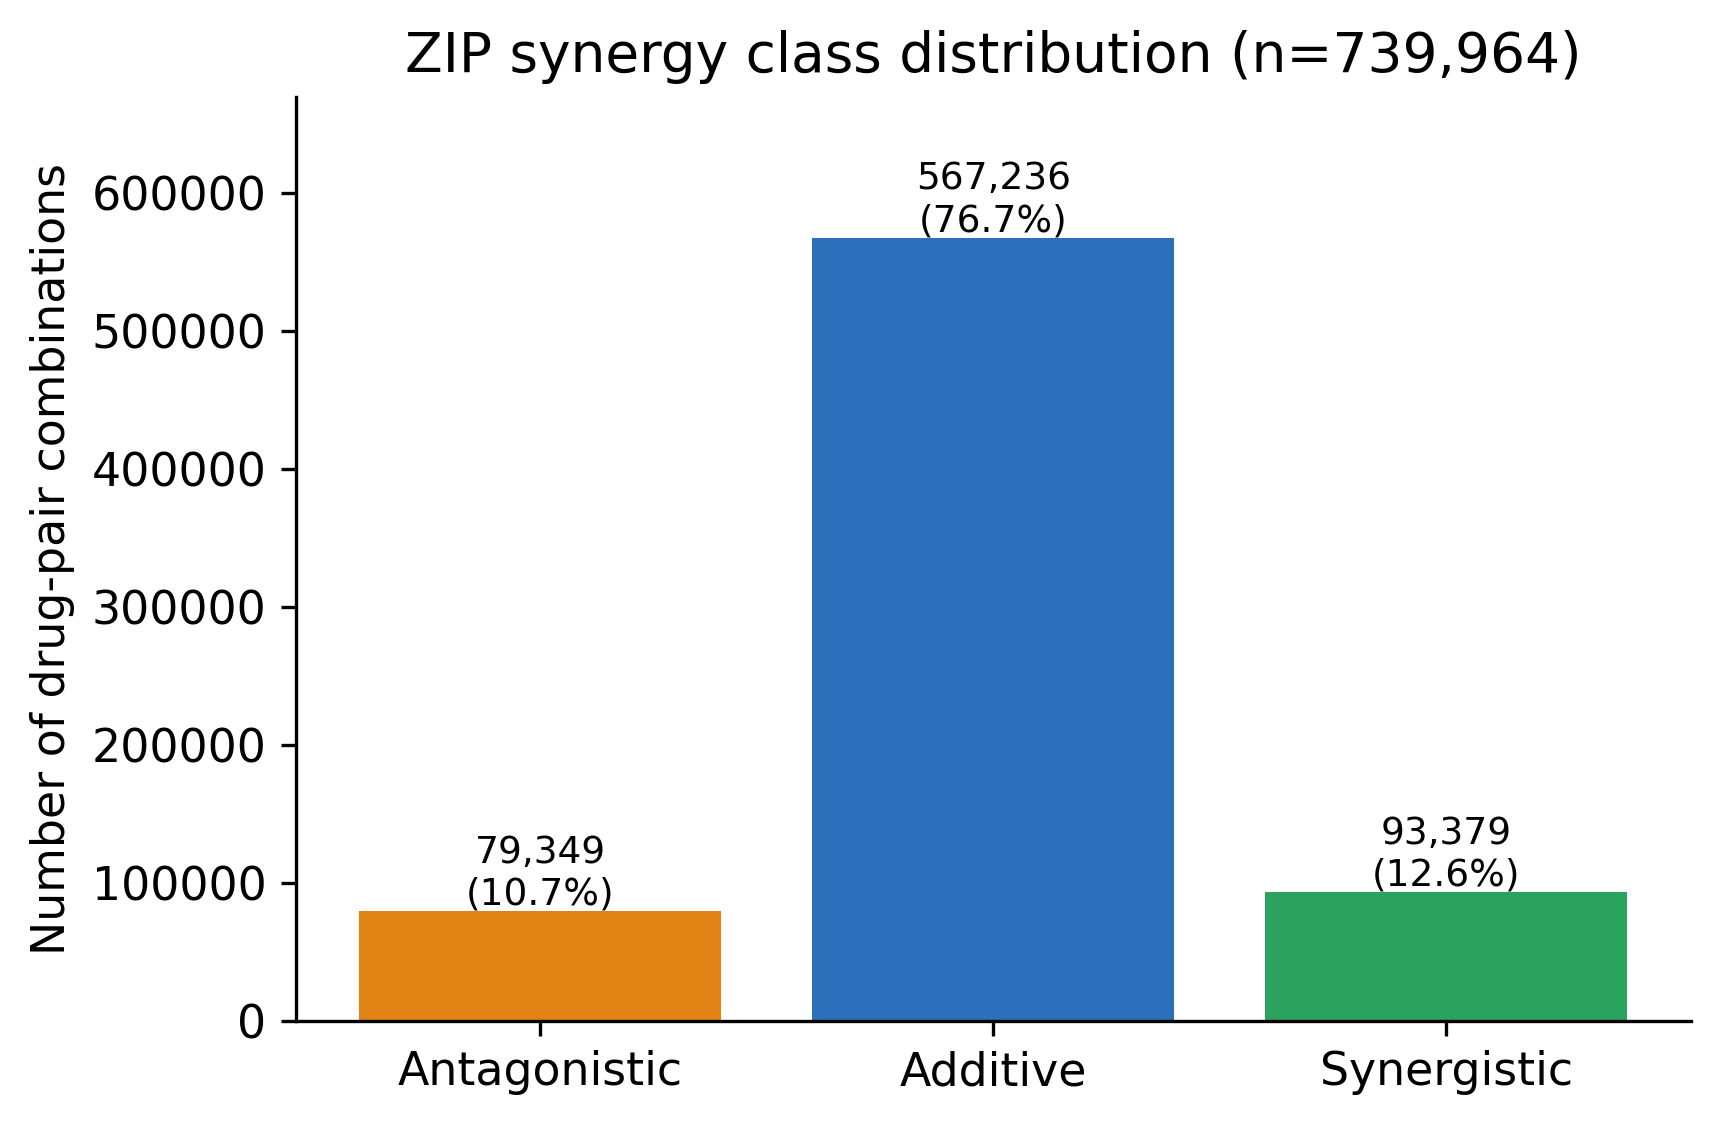
\includegraphics[width=0.62\textwidth]{fig1_class_distribution.png}
\caption{Distribution of ZIP synergy classes across all $739{,}964$ combinations. Additive pairs
dominate; synergistic and antagonistic combinations each form roughly one-eighth of the data.}
\label{fig:dist}
\end{figure}

\subsection{Overall performance on the standard split}
Table~\ref{tab:overall} summarizes test performance with bootstrap confidence intervals. LightGBM
outperforms the logistic baseline on every metric, and by a wide margin on the class-balanced ones.
Although its raw accuracy ($0.782$) is only modestly above the $0.766$ majority baseline, its balanced
accuracy ($0.805$) and macro-F1 ($0.703$) far exceed the baseline's $0.333$ and $0.289$, showing the
headline accuracy comes from recovering minority classes rather than defaulting to the majority. The
confidence intervals for the two models do not overlap on any metric, and a McNemar test is decisive:
LightGBM is uniquely correct on $9{,}941$ test cases versus $3{,}130$ for logistic regression
($\chi^2 = 3548$, $p<0.001$).

\begin{table}[H]
\centering
\caption{Standard-split test performance ($73{,}618$ combinations) with $95\%$ bootstrap confidence
intervals. Best value per row in bold.}
\label{tab:overall}
\small
\begin{tabular}{lccc}
\toprule
Metric & Majority baseline & Logistic Regression & LightGBM \\
\midrule
Accuracy          & $0.766$ & $0.689\ [0.686,0.692]$ & $\mathbf{0.782}\ [0.779,0.785]$ \\
Balanced accuracy & $0.333$ & $0.633\ [0.629,0.639]$ & $\mathbf{0.805}\ [0.801,0.809]$ \\
Macro-F1          & $0.289$ & $0.559\ [0.555,0.564]$ & $\mathbf{0.703}\ [0.699,0.706]$ \\
Cohen's $\kappa$  & $0.000$ & $0.373\ [0.367,0.379]$ & $\mathbf{0.545}\ [0.540,0.551]$ \\
Macro AUC (OvR)   & ---     & $0.821\ [0.818,0.824]$ & $\mathbf{0.922}\ [0.920,0.924]$ \\
\bottomrule
\end{tabular}
\end{table}

\subsection{Per-class behavior}
The per-class breakdown (Table~\ref{tab:perclass}) and confusion matrices (Figure~\ref{fig:cm}) show
where the models succeed. With class re-weighting, LightGBM recovers the rare classes at high
recall---$84.1\%$ of antagonistic and $80.5\%$ of synergistic pairs---while keeping $77.0\%$ recall and
$94.9\%$ precision on additive pairs. The cost is moderate precision on the rare classes
($0.52$ antagonistic, $0.49$ synergistic): some additive pairs are flagged as interacting.

Because the classes are ordinal, we quantify the error structure rather than reading it off the
confusion matrix (Table~\ref{tab:ordinal}). Only $4.6\%$ of LightGBM's errors span the full ordinal
distance---a synergistic pair called antagonistic, or the reverse---against $14.1\%$ for a prior-only
predictor and $16.1\%$ for the logistic baseline, and the mean absolute ordinal distance is lowest for
LightGBM ($0.228$). The ranked probability score orders the models consistently ($0.070$ for LightGBM
against $0.111$ for logistic regression and $0.103$ for the global prior). The claim that residual
errors are predominantly interacting-versus-additive rather than between opposite interaction types is
therefore supported quantitatively---an encouraging pattern for triage. We note that the
per-(cell line, drug) memorization baseline attains a marginally better ranked probability score
($0.067$) than the full model, consistent with the finding that most of the signal is conditional base
rates.

\begin{table}[H]
\centering
\caption{Ordinal error structure on the standard test split. RPS is the ranked probability score
(lower is better); MAOD is the mean absolute ordinal distance; a distance-two error confuses the two
opposite interaction types.}
\label{tab:ordinal}
\small
\begin{tabular}{lcccc}
\toprule
Model & RPS & MAOD & Distance-2 errors & Share of errors at distance 2 \\
\midrule
Global prior (reference)      & $0.1032$ & $1.0169$ & $9{,}234$ & $14.1\%$ \\
Logistic regression           & $0.1106$ & $0.3606$ & $3{,}671$ & $16.1\%$ \\
Per-(cell line, drug) prior   & $\mathbf{0.0674}$ & $0.2900$ & $795$ & $\mathbf{3.9\%}$ \\
LightGBM                      & $0.0702$ & $\mathbf{0.2282}$ & $\mathbf{738}$ & $4.6\%$ \\
\bottomrule
\end{tabular}
\end{table}

\begin{table}[H]
\centering
\caption{Per-class precision, recall and F1 on the standard test split.}
\label{tab:perclass}
\small
\begin{tabular}{llcccc}
\toprule
Class & Model & Precision & Recall & F1 & Support \\
\midrule
\multirow{2}{*}{Antagonistic} & LightGBM & $0.524$ & $0.841$ & $0.646$ & $7{,}989$ \\
                              & Logistic & $0.354$ & $0.574$ & $0.438$ & $7{,}989$ \\
\addlinespace
\multirow{2}{*}{Additive}     & LightGBM & $0.949$ & $0.770$ & $0.850$ & $56{,}395$ \\
                              & Logistic & $0.923$ & $0.719$ & $0.809$ & $56{,}395$ \\
\addlinespace
\multirow{2}{*}{Synergistic}  & LightGBM & $0.493$ & $0.805$ & $0.612$ & $9{,}234$ \\
                              & Logistic & $0.334$ & $0.607$ & $0.431$ & $9{,}234$ \\
\bottomrule
\end{tabular}
\end{table}

\begin{figure}[H]
\centering
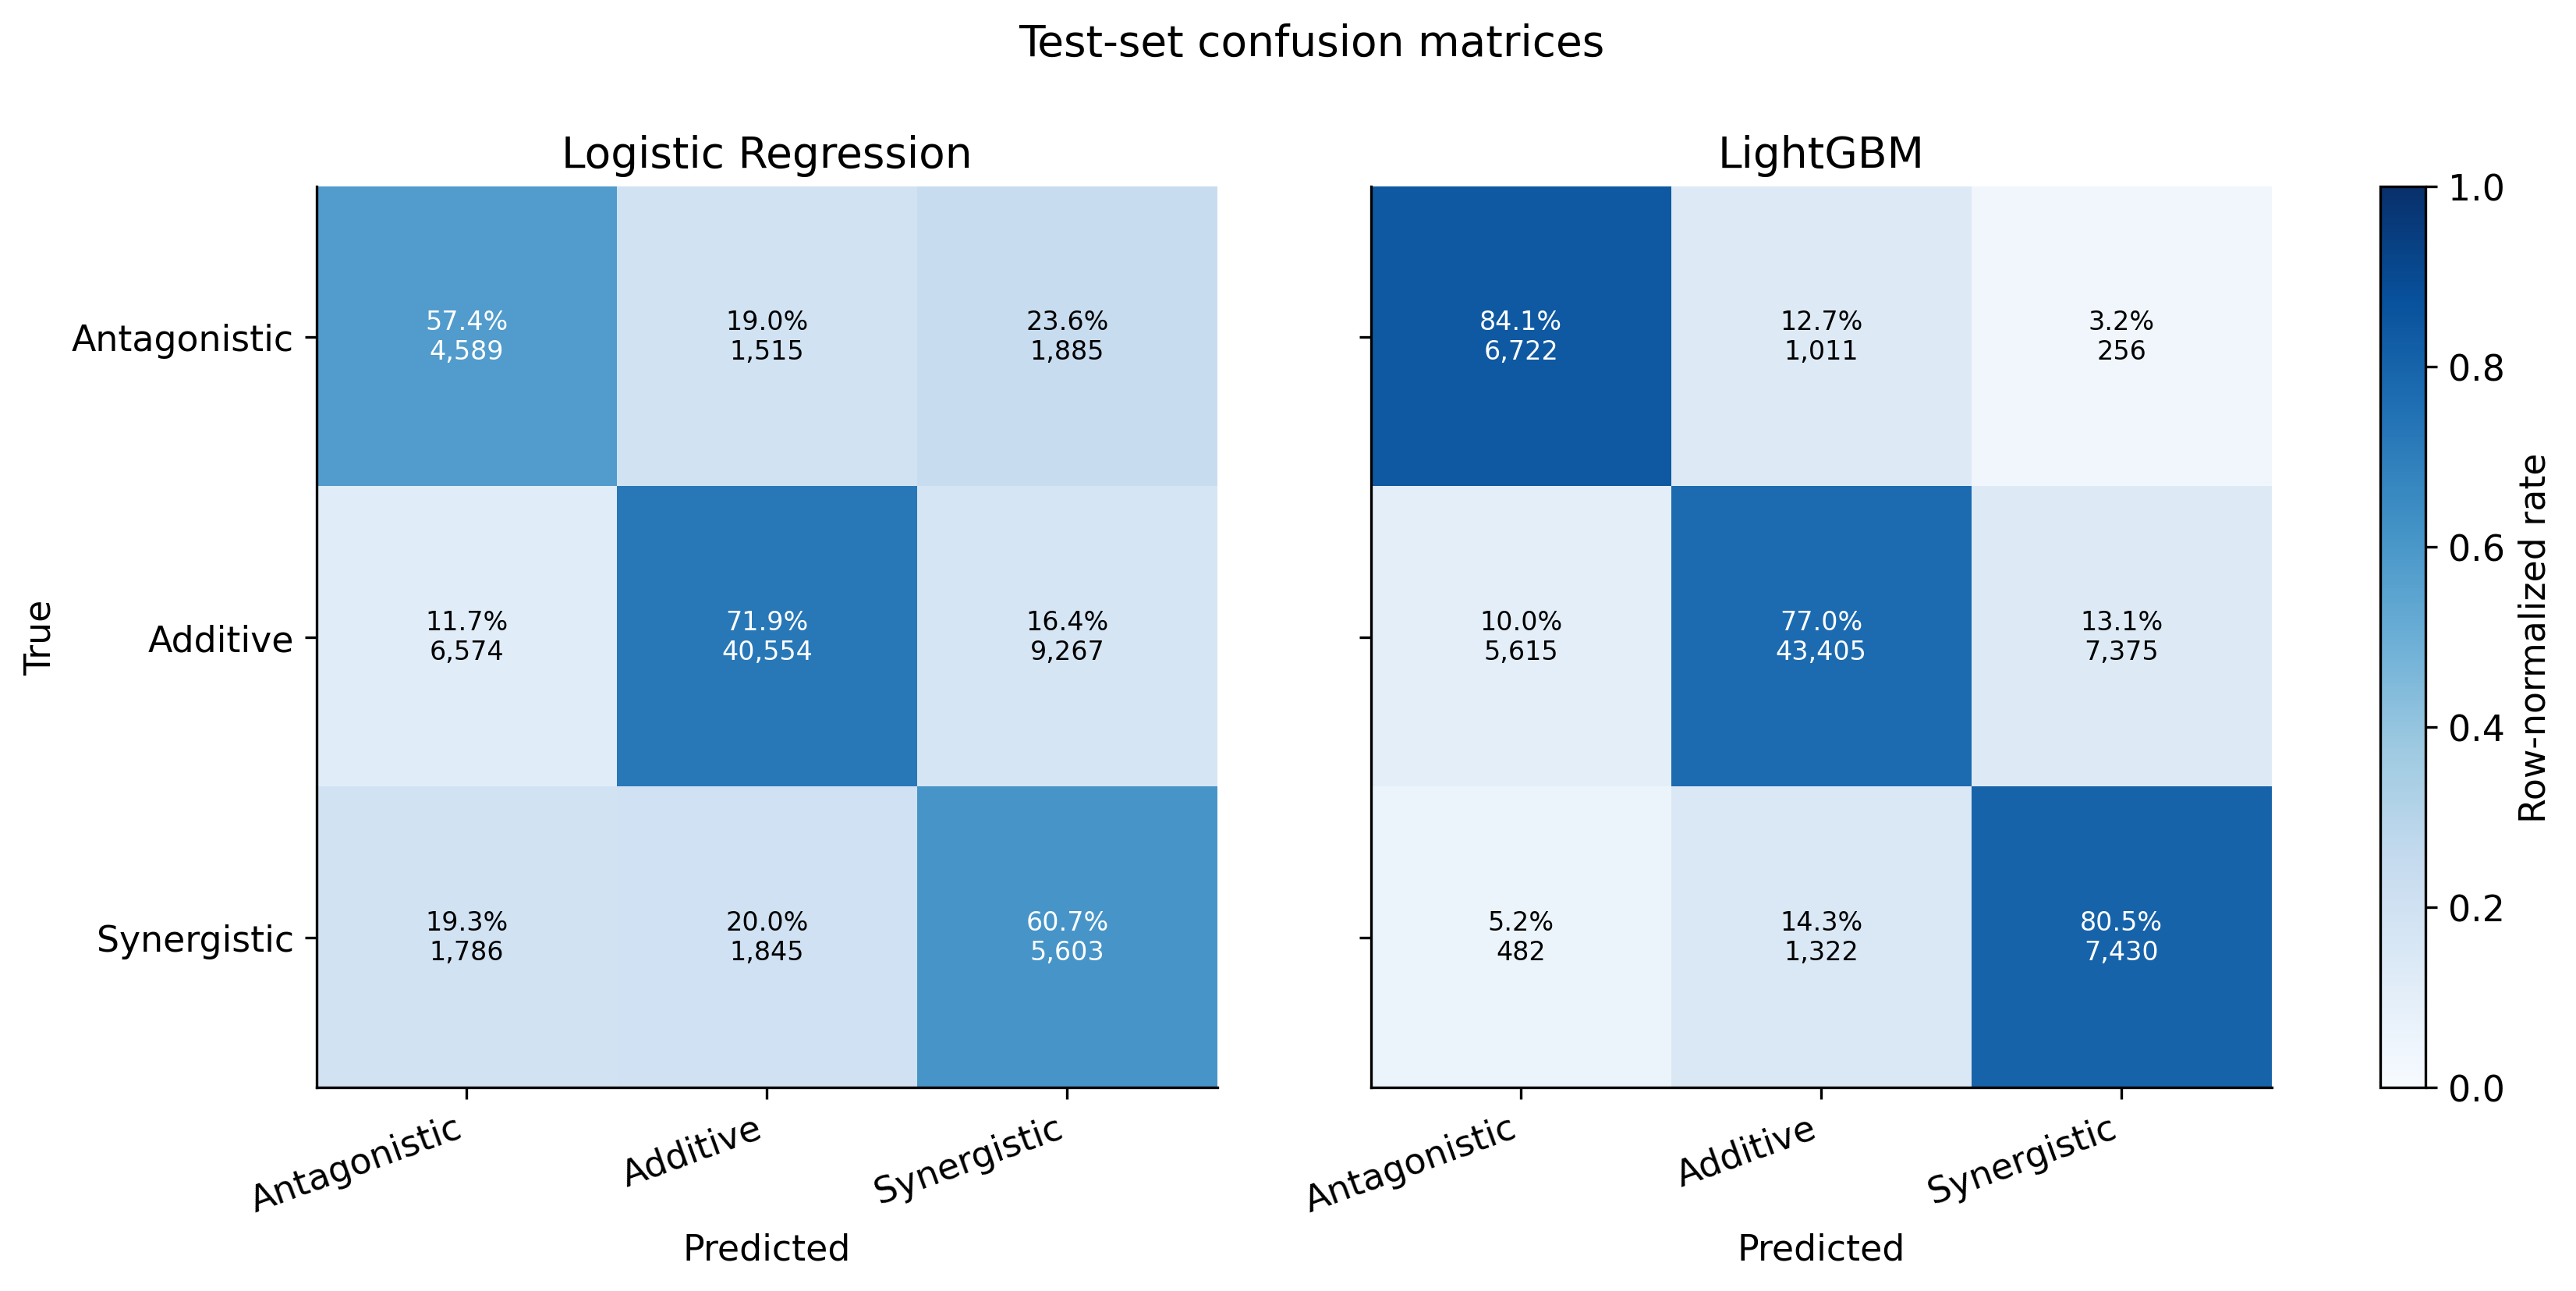
\includegraphics[width=0.95\textwidth]{fig2_confusion_matrices.png}
\caption{Row-normalized confusion matrices. LightGBM (right) places far more mass on the diagonal for
the rare classes than the logistic baseline (left).}
\label{fig:cm}
\end{figure}

\subsection{Precision--recall and calibration}
Because ROC-AUC is optimistic under strong imbalance, we report precision--recall analysis
(Figure~\ref{fig:pr}). LightGBM achieves AUPRC of $0.71$ (antagonistic) and $0.72$ (synergistic),
against class priors of $0.11$ and $0.13$---roughly a six-fold enrichment---and $0.96$ for additive.
The logistic baseline trails substantially on the minority classes ($0.48$ and $0.37$).

Calibration is assessed for both models rather than described qualitatively
(Figure~\ref{fig:cal}, Table~\ref{tab:calib}). LightGBM's top-label expected calibration error is
$0.024$ with a multiclass Brier score of $0.291$, against $0.111$ and $0.449$ for the logistic
baseline: the gradient-boosted probabilities are roughly five times better calibrated on the top-label
statistic. Calibration is nonetheless clearly worse for the rare classes, whose one-vs-rest calibration
errors are $0.079$ (antagonistic) and $0.086$ (synergistic) against $0.024$ overall, and the reliability
curves for those classes lie below the diagonal, confirming that class re-weighting inflates rare-class
probabilities. Post-hoc recalibration would therefore be advisable before the scores are used as
absolute risks. For reference, the global prior is trivially well calibrated (ECE $0.001$) while being
useless as a predictor (Brier $0.386$, mean ordinal distance $1.017$), which is why calibration must be
read alongside discrimination.

\begin{table}[H]
\centering
\caption{Calibration on the standard test split. ECE uses $15$ uniform bins; per-class values are
one-vs-rest. Brier is the multiclass score. Lower is better throughout.}
\label{tab:calib}
\small
\begin{tabular}{lcccc}
\toprule
Model & Top-label ECE & Brier & ECE antagonistic & ECE synergistic \\
\midrule
Global prior (reference)     & $0.0009$ & $0.3857$ & $0.0014$ & $0.0005$ \\
Logistic regression          & $0.1108$ & $0.4488$ & $0.1488$ & $0.1501$ \\
Per-(cell line, drug) prior  & $0.0442$ & $\mathbf{0.2534}$ & $0.0472$ & $0.0572$ \\
LightGBM                     & $\mathbf{0.0236}$ & $0.2905$ & $0.0786$ & $0.0855$ \\
\bottomrule
\end{tabular}
\end{table}

\begin{figure}[H]
\centering
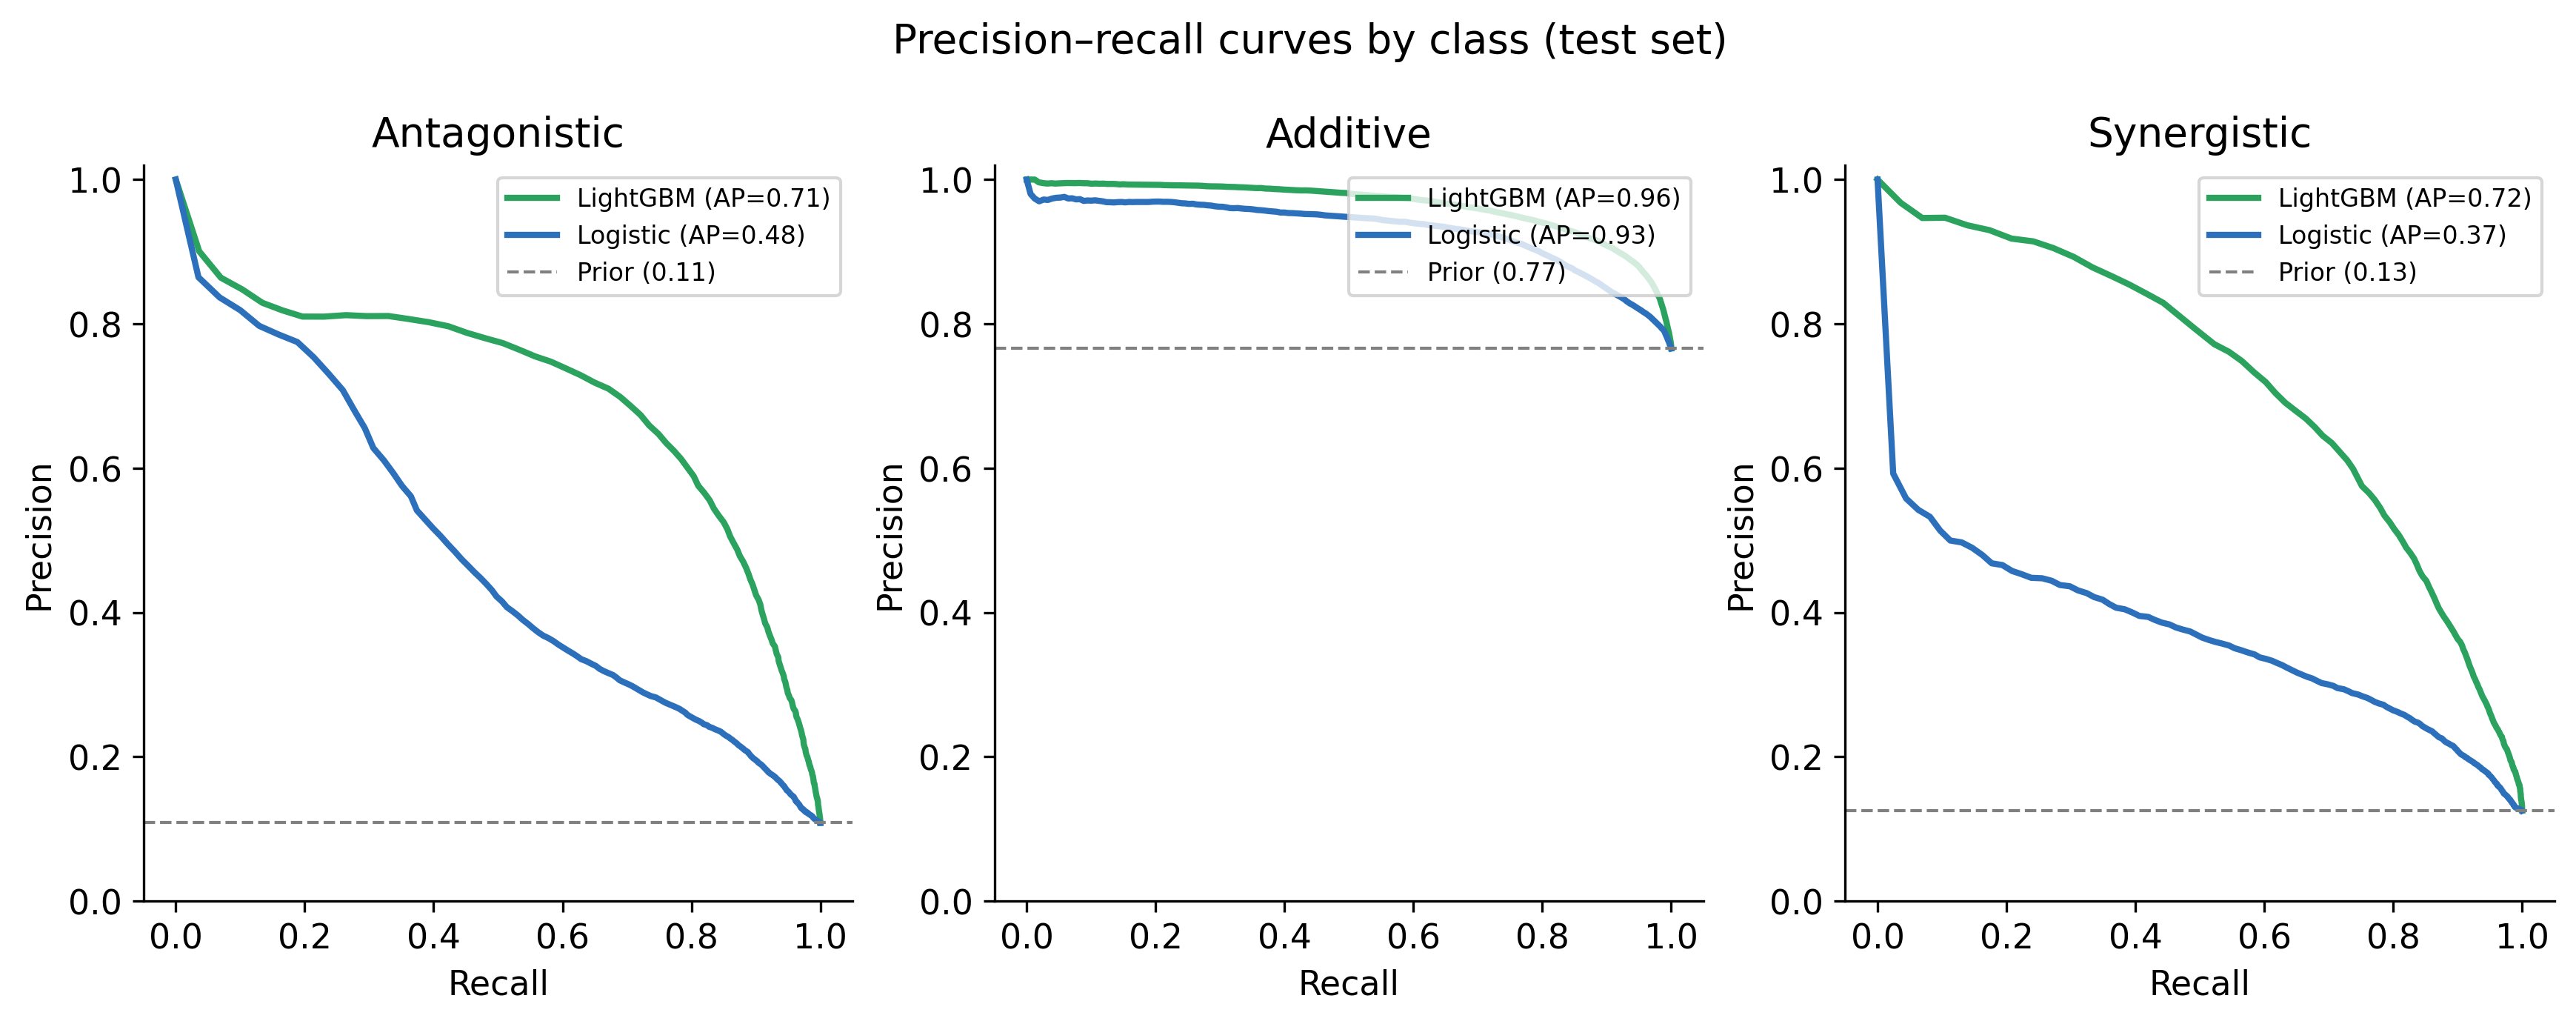
\includegraphics[width=0.98\textwidth]{fig7_pr_curves.png}
\caption{Per-class precision--recall curves on the standard test split, with average precision (AP) and
the class prior (dashed). LightGBM enriches the rare classes roughly six-fold over their priors.}
\label{fig:pr}
\end{figure}

\begin{figure}[H]
\centering
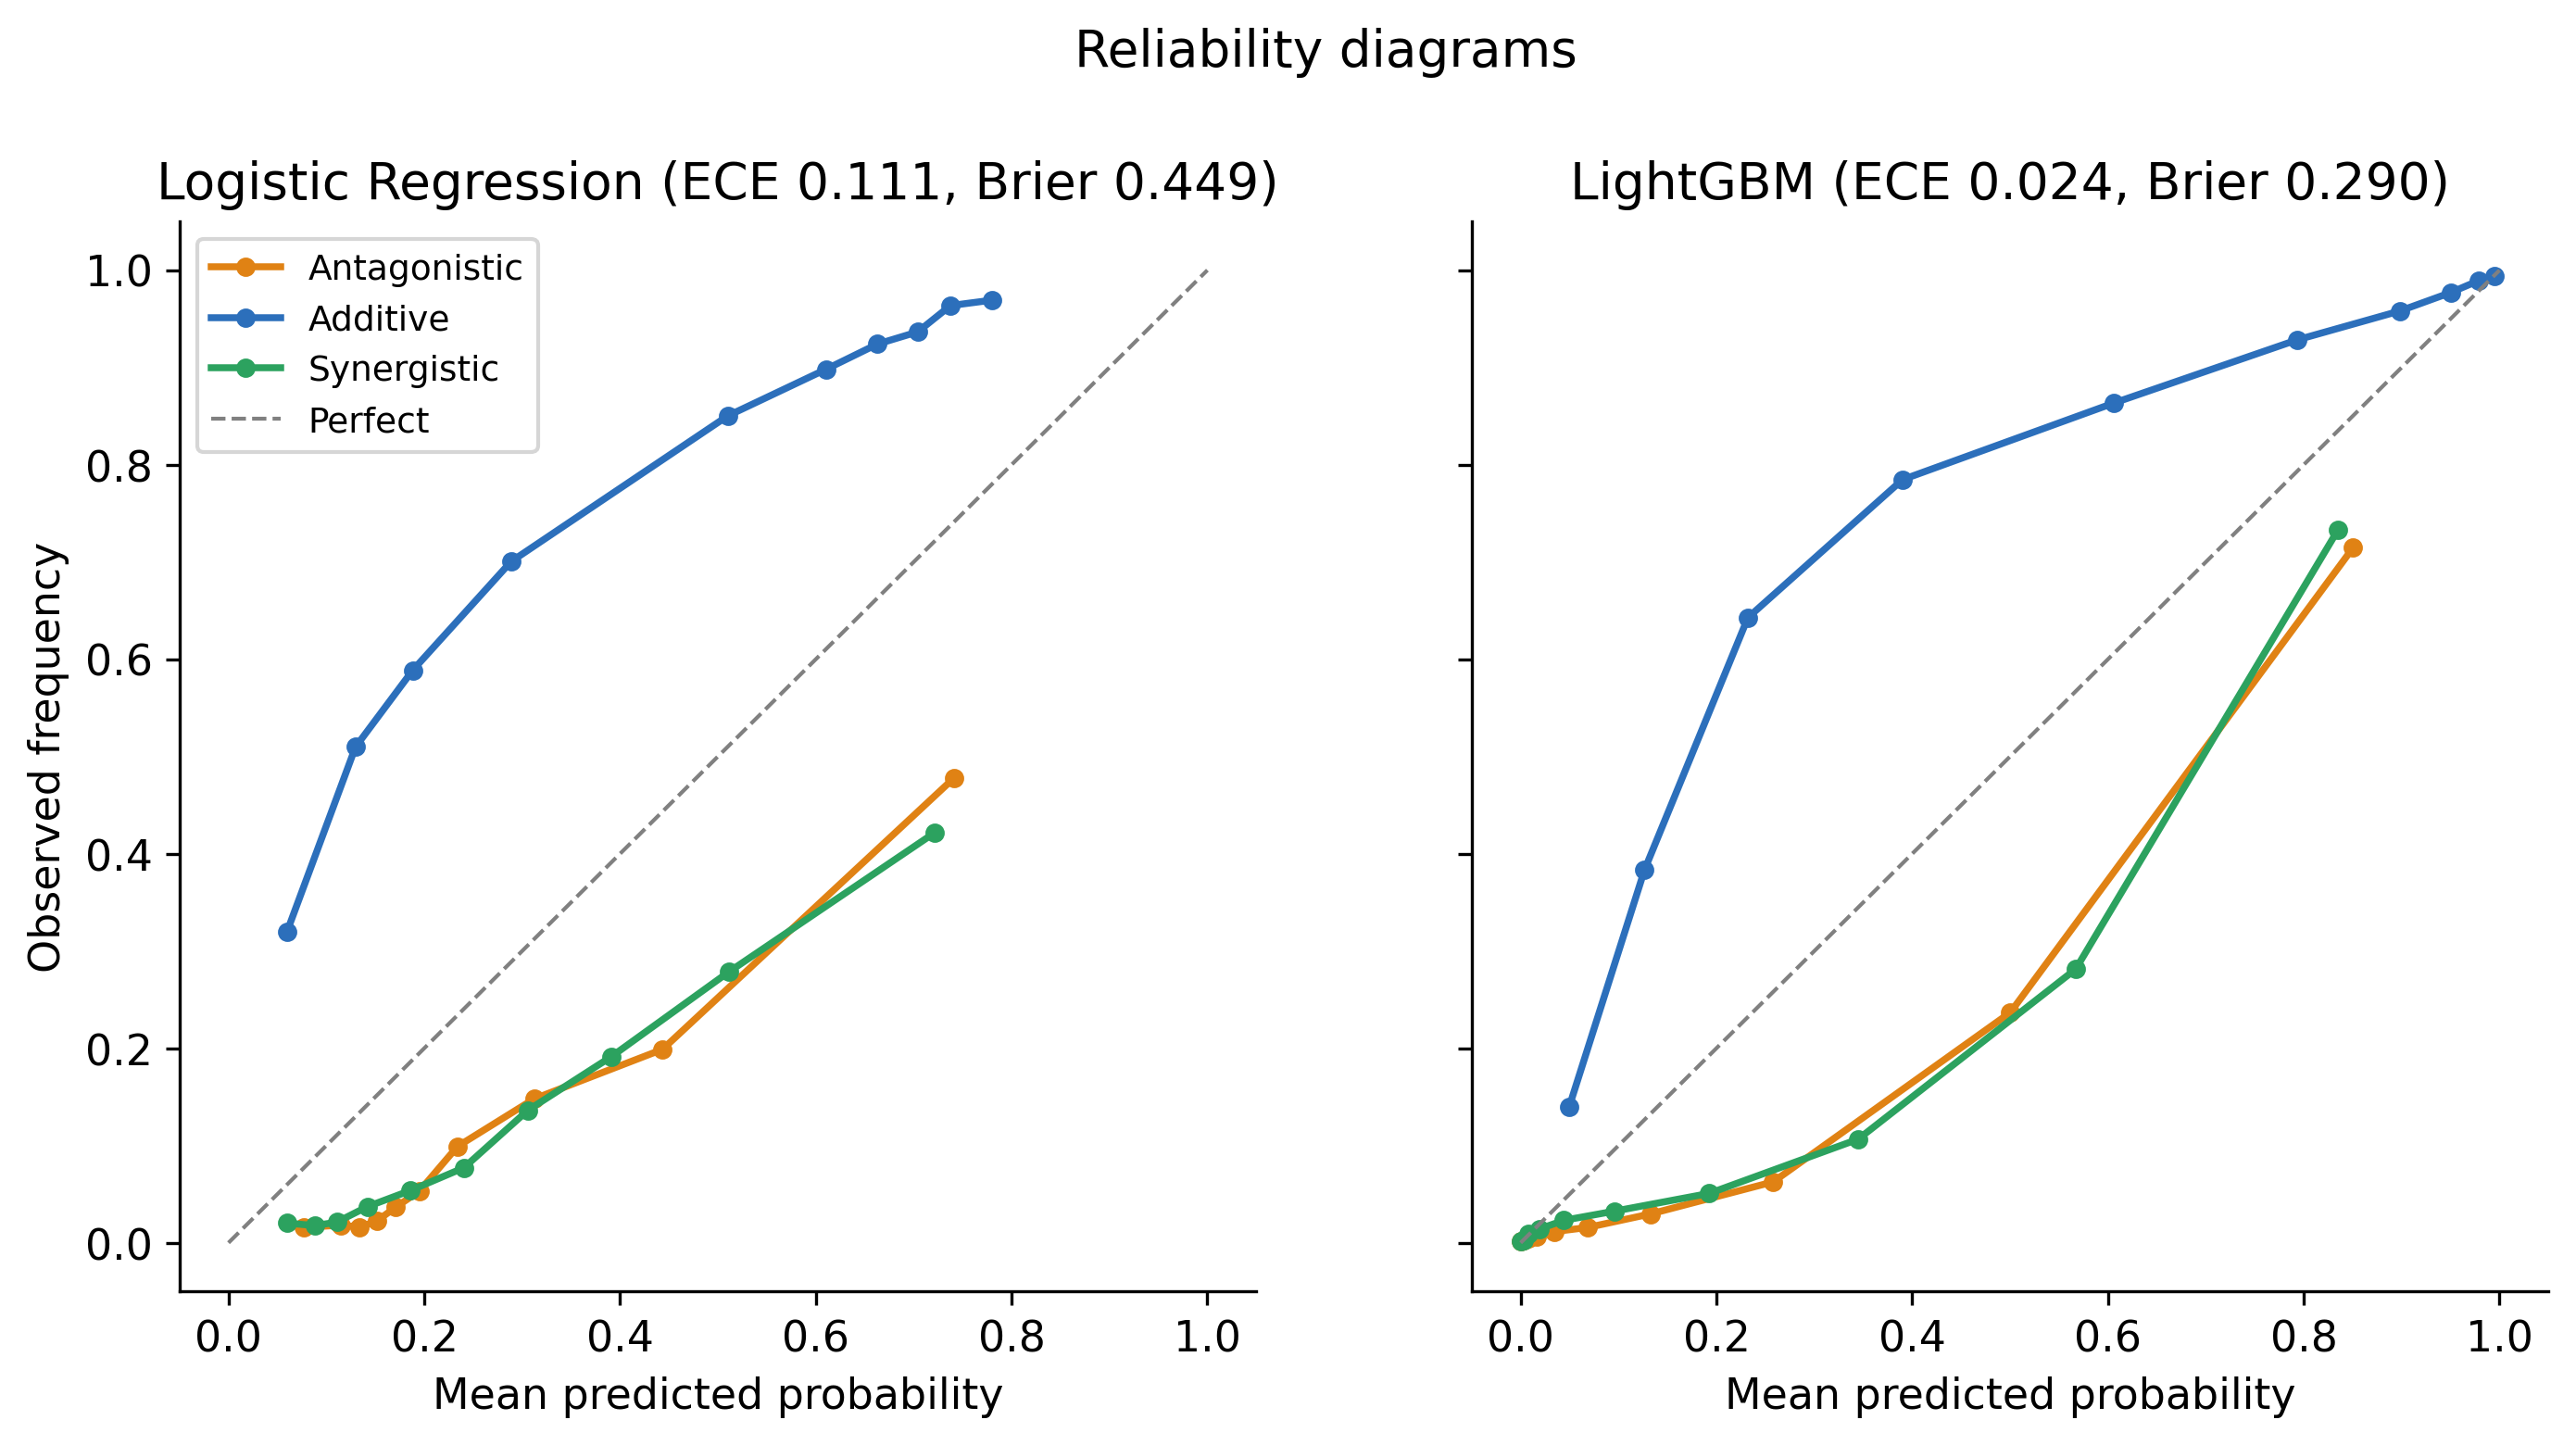
\includegraphics[width=0.5\textwidth]{fig11_calibration.png}
\caption{Reliability diagrams for both models, with expected calibration error and multiclass Brier
score in each panel title. LightGBM (right) is substantially better calibrated than the logistic
baseline (left); in both models the re-weighted rare classes lie below the diagonal, indicating
over-confidence.}
\label{fig:cal}
\end{figure}

\subsection{Feature importance}
Permutation importance (Figure~\ref{fig:perm}), which unlike impurity- or split-gain-based importance
is not biased toward high-cardinality variables, identifies the
\emph{cell line} as the single most informative feature (macro-F1 drop $0.247$ when shuffled), ahead
of the two drug identities ($0.128$ and $0.115$) and the study ($0.017$). Notably, this re-orders the
naive gain-based ranking, in which the high-cardinality drug fields appeared dominant---illustrating
why cardinality-robust attribution matters. The engineered target and clinical-phase descriptors
contribute little in this feature set. Tissue appears to contribute nothing (drop $-0.004$), but this
is a masking artefact rather than irrelevance: permutation importance is not robust to correlated
features, and every cell line in the dataset maps to exactly one tissue, so permuting tissue alone
leaves cell-line identity intact as a perfect proxy. Permuting the two jointly gives a drop of $0.256$,
which exceeds the sum of the individual drops ($0.243$). Tissue is therefore genuinely redundant
\emph{given} the cell line---a deterministic relation---rather than uninformative in itself. Study
identity contributes modestly; because it can encode assay platform and curation effects, it should be
treated as a potential confounder rather than a purely biological predictor. The primacy of cell line
foreshadows the cold-start result below: the model relies heavily on having seen the cellular
background during training.

\begin{figure}[H]
\centering
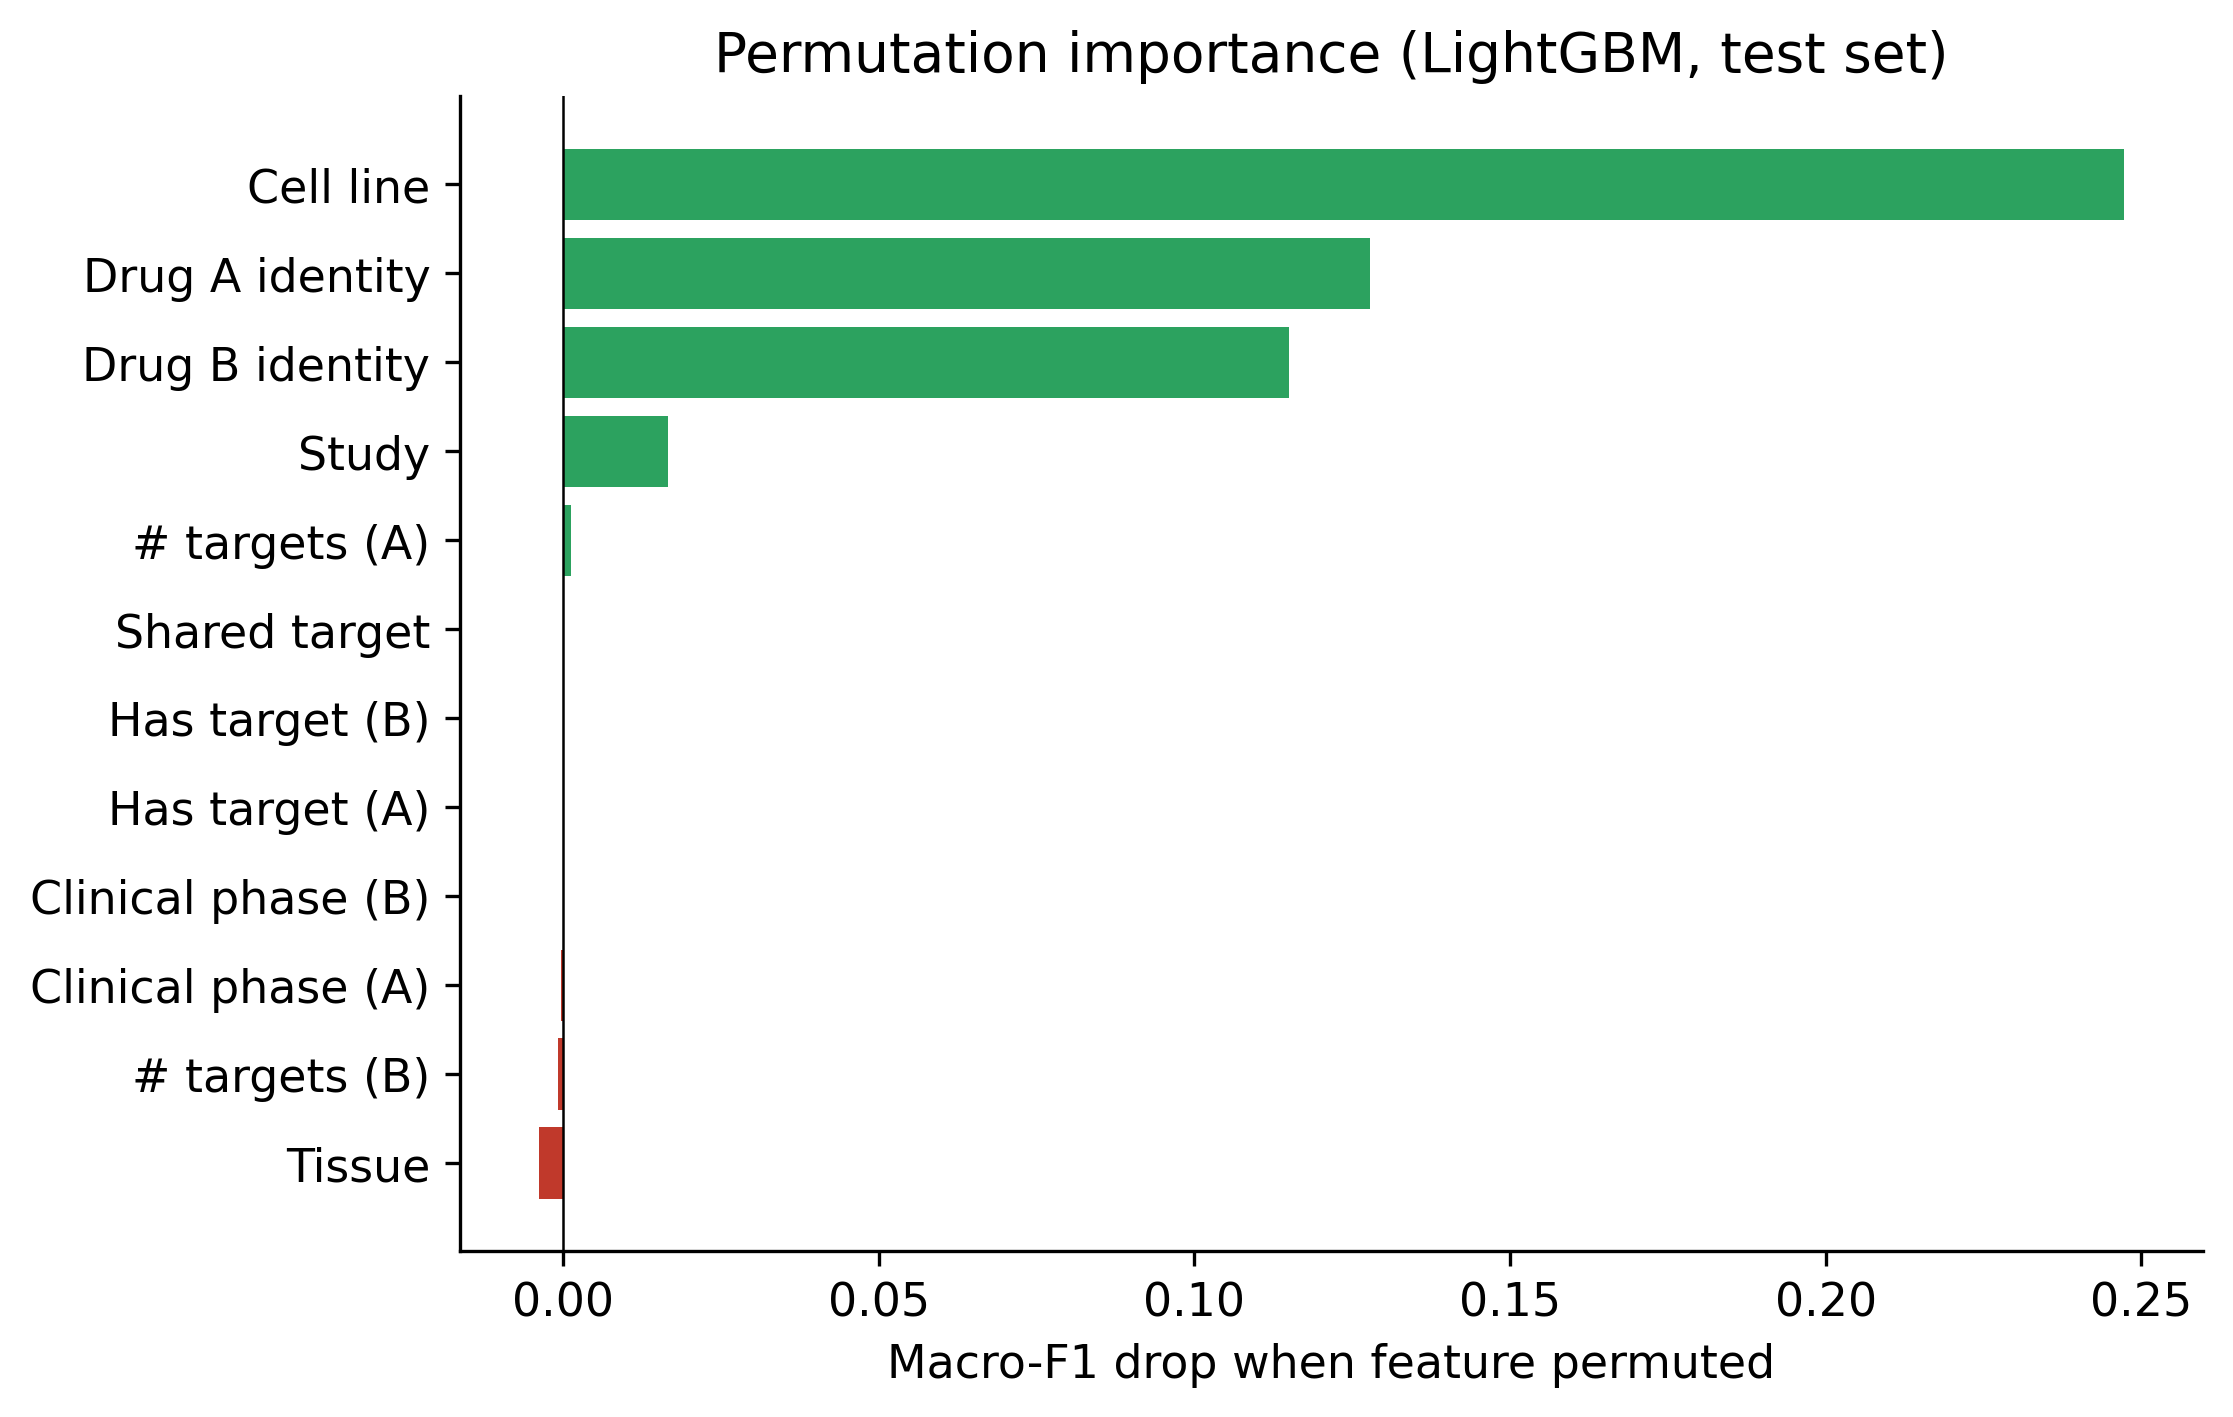
\includegraphics[width=0.72\textwidth]{fig8_permutation_importance.png}
\caption{Permutation importance (decrease in macro-F1 when each feature is shuffled). Cell line
dominates, followed by the two drug identities; coarse target and clinical-phase descriptors contribute
little in this feature set.}
\label{fig:perm}
\end{figure}

\subsection{Cold-start generalization}
The central new result concerns distribution shift (Figure~\ref{fig:cold}, Table~\ref{tab:cold}). When
the test set involves drugs unseen in training, LightGBM's balanced accuracy falls from $0.805$ to
$0.694$ and macro-F1 from $0.703$ to $0.631$---a clear but graceful degradation: the model still
recovers most antagonistic ($70\%$) and a majority of synergistic ($59\%$) pairs, indicating some
genuine transfer through cell-context and target features. When the test set involves \emph{unseen
cell lines}, however, performance collapses: balanced accuracy drops to $0.482$, barely above the
$0.333$ random floor, with antagonistic recall falling to $0.20$. In other words, the strong
standard-split numbers are substantially carried by memorization of per-cell-line synergy base rates,
and the model has limited ability to generalize to a cellular background it has never seen. This is the
gap that molecular and omics features would need to close, and it is invisible to the conventional
split.

\begin{figure}[H]
\centering
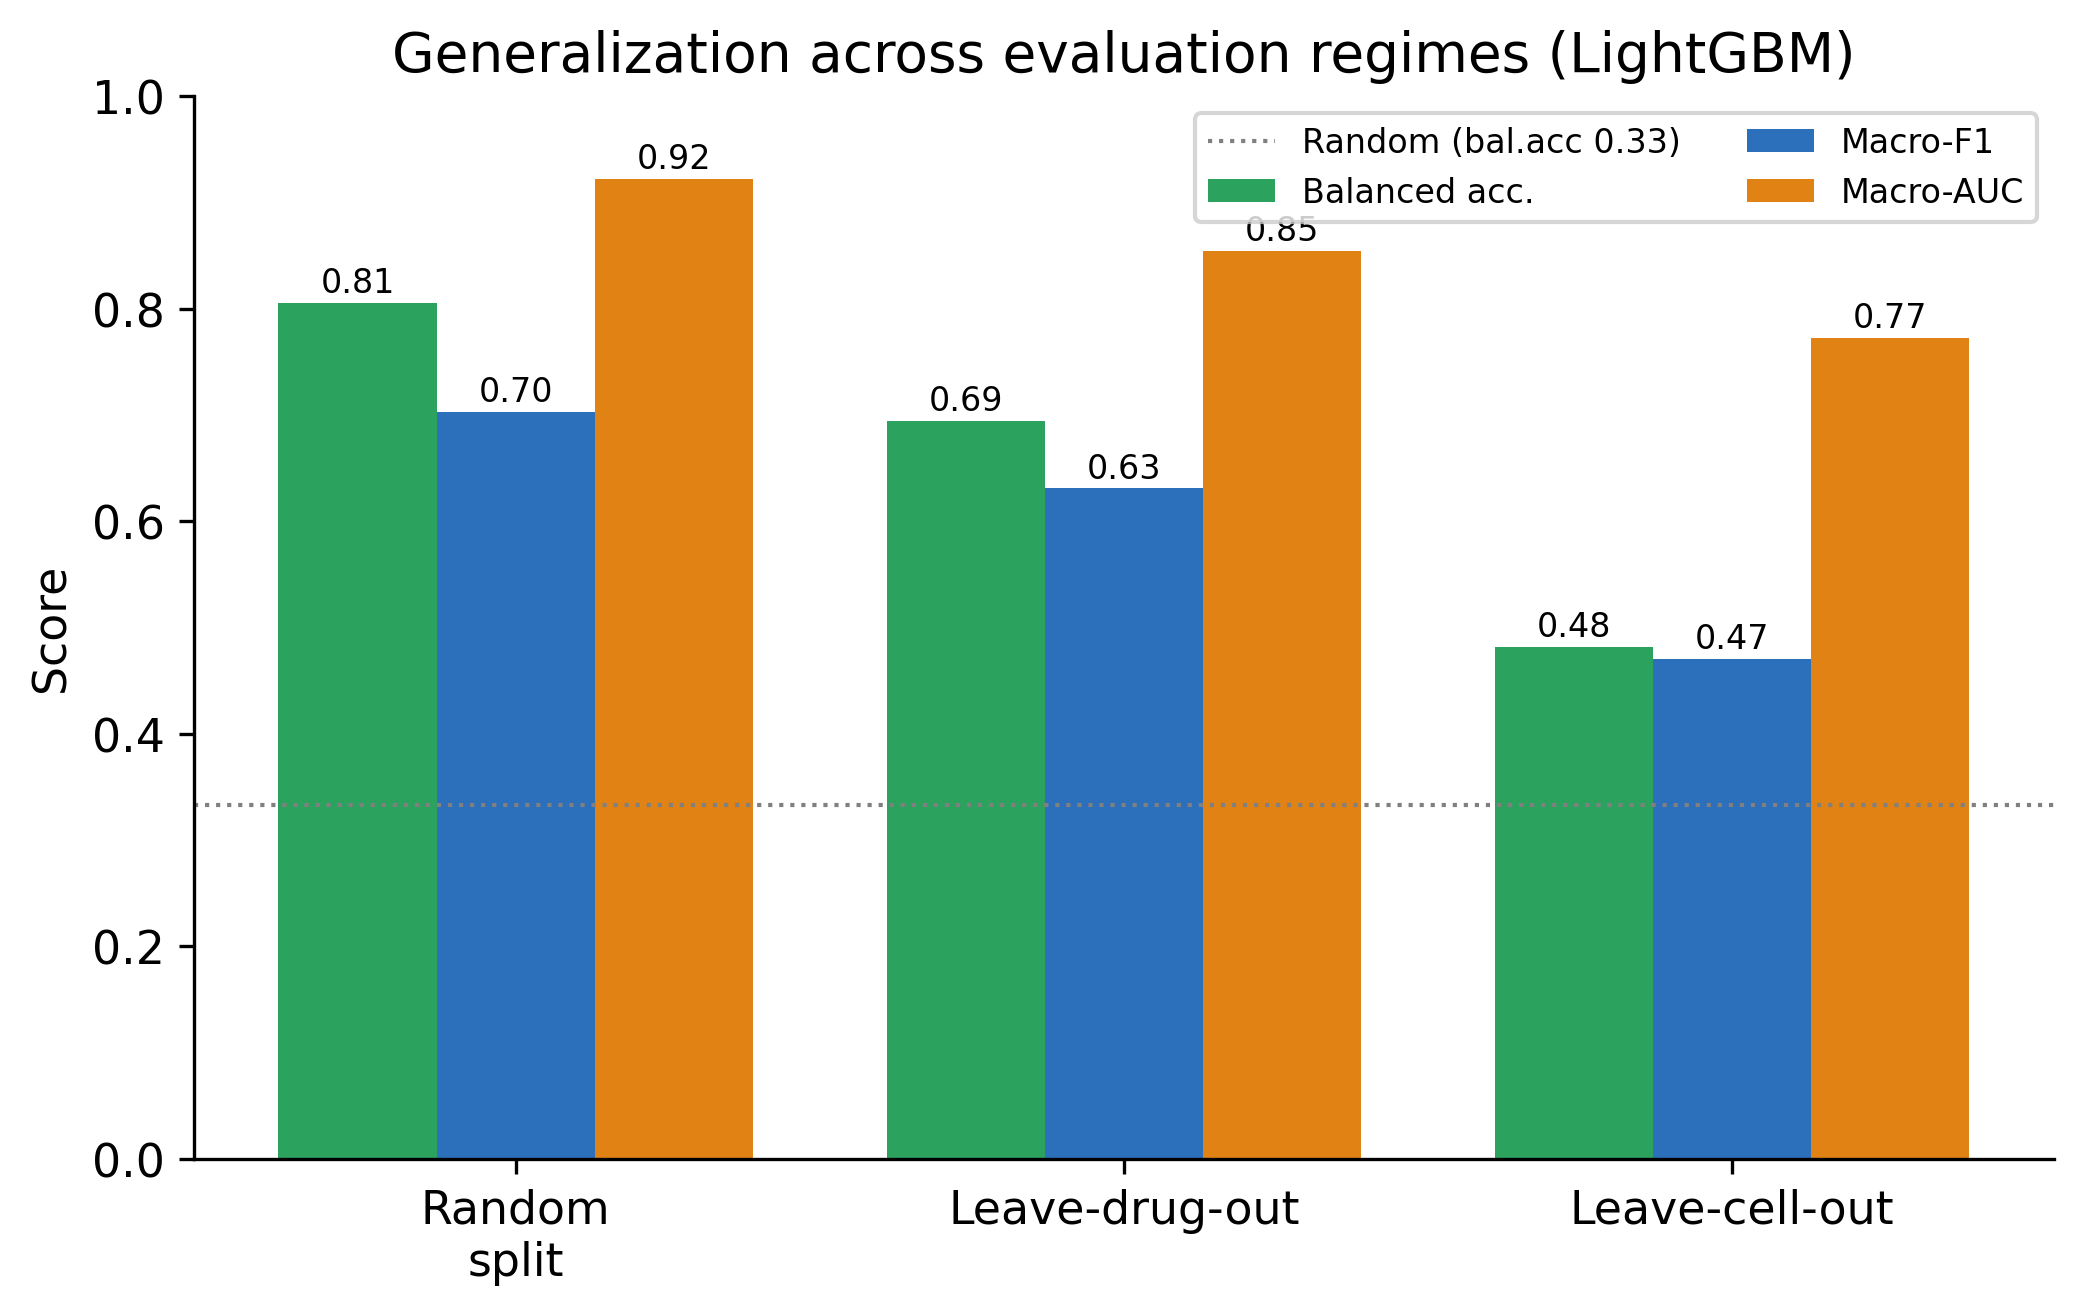
\includegraphics[width=0.72\textwidth]{fig9_coldstart.png}
\caption{LightGBM generalization across the three regimes. Performance degrades for unseen drugs and
collapses toward the random floor for unseen cell lines.}
\label{fig:cold}
\end{figure}

\begin{table}[H]
\centering
\caption{LightGBM performance across evaluation regimes, with per-class recall.}
\label{tab:cold}
\small
\begin{tabular}{lcccccc}
\toprule
 & & & & \multicolumn{3}{c}{Recall} \\
\cmidrule(lr){5-7}
Regime & Bal.\ acc. & Macro-F1 & Macro-AUC & Antag. & Add. & Syn. \\
\midrule
Standard (grouped) & $\mathbf{0.805}$ & $\mathbf{0.703}$ & $\mathbf{0.922}$ & $0.841$ & $0.770$ & $0.805$ \\
Leave-drug-out     & $0.694$ & $0.631$ & $0.855$ & $0.696$ & $0.792$ & $0.594$ \\
Leave-cell-line-out& $0.482$ & $0.470$ & $0.773$ & $0.196$ & $0.804$ & $0.445$ \\
\bottomrule
\end{tabular}
\end{table}

\subsection{Study confounder and cross-study/tissue transfer}
Three further experiments probe whether the standard-split performance depends on the study confounder
and how far it transfers across whole studies and tissues (Table~\ref{tab:robust}). First, a no-study
ablation---retraining with the study feature removed---leaves standard-split performance essentially
unchanged (balanced accuracy $0.807\rightarrow0.806$, macro-F1 unchanged at $0.708$), so the reported
numbers are not an artefact of study-level platform or curation signal. Second, under leave-study-out
evaluation, where $14$ of the $26$ studies (including NCI-ALMANAC) are held out entirely, performance
collapses to the random floor (balanced accuracy $0.332$, macro one-vs-rest AUC $0.421$), with the
model defaulting almost entirely to the additive class (synergistic recall $0.01$). Third,
leave-tissue-out evaluation ($7$ of $17$ tissues held out) gives balanced accuracy $0.431$ and AUC
$0.772$---a collapse comparable to the leave-cell-line-out regime. Together these results show
essentially no transfer to unseen studies and limited transfer to unseen tissues, confirming that the
strong standard-split numbers reflect entity- and context-specific base rates rather than mechanism,
while ruling out the study identifier itself as the driver.

\begin{table}[H]
\centering
\caption{Robustness experiments (LightGBM, fixed seed $42$): no-study ablation on the standard split,
and transfer to entirely unseen studies and tissues. Held-out counts are given as (held/total).}
\label{tab:robust}
\small
\begin{tabular}{lcccccc}
\toprule
 & & & & \multicolumn{3}{c}{Recall} \\
\cmidrule(lr){5-7}
Regime & Bal.\ acc. & Macro-F1 & Macro-AUC & Antag. & Add. & Syn. \\
\midrule
Standard, with study      & $0.807$ & $0.708$ & $0.923$ & $0.840$ & $0.778$ & $0.802$ \\
Standard, no study        & $0.806$ & $0.708$ & $0.922$ & $0.838$ & $0.778$ & $0.803$ \\
Leave-study-out ($14/26$) & $0.332$ & $0.312$ & $0.421$ & $0.000$ & $0.985$ & $0.010$ \\
Leave-tissue-out ($7/17$) & $0.431$ & $0.466$ & $0.772$ & $0.149$ & $0.976$ & $0.169$ \\
\bottomrule
\end{tabular}
\end{table}

\subsection{What the gradient-boosted model adds over memorization}
To establish how much of the performance is recoverable from entity base rates alone, we compared the
model against a graded series of lookup baselines that do no learning beyond counting training labels
(Table~\ref{tab:baselines}). Each is fitted on the training partition only, smoothed toward the global
prior with pseudo-count $20$, and backs off to a coarser level for unseen keys; hard predictions apply
the same inverse-frequency class weights used in training, so the comparison is like-for-like.

Two things follow. First, the interaction between compound and cellular context is genuinely necessary:
every additive predictor plateaus between $0.60$ and $0.65$ balanced accuracy---single-entity priors
($0.598$ for cell line, $0.611$ for drug pair), the linear baseline ($0.633$) and a depth-one LightGBM
that cannot represent any feature interaction by construction ($0.653$). Performance rises only when
drug and cell-line identity are combined. Second, and more soberingly, that interaction is almost
entirely captured by memorization: a per-(cell line, drug) base-rate table reaches $0.778$ balanced
accuracy and $0.895$ macro-AUC, so the full gradient-boosted model contributes only a further $0.027$
on each measure. The headline result should therefore be understood as conditional base-rate recall
rather than as evidence that the model has learned pharmacological interaction, which is precisely what
the cold-start collapse in the following sections would predict.

\begin{table}[H]
\centering
\caption{Memorization baselines on the standard test split. Lookup baselines are smoothed training-set
class frequencies with back-off; no model is fitted. ``Interactions'' indicates whether the predictor
can represent a drug-by-context term.}
\label{tab:baselines}
\small
\begin{tabular}{lcccl}
\toprule
Predictor & Bal.\ acc. & Macro-F1 & Macro-AUC & Interactions \\
\midrule
Global class prior                       & $0.333$ & $0.065$ & $0.500$ & none \\
Per-cell-line prior                      & $0.598$ & $0.516$ & $0.799$ & none \\
Per-drug-pair prior                      & $0.611$ & $0.510$ & $0.782$ & none \\
Logistic regression (baseline model)     & $0.633$ & $0.559$ & $0.821$ & additive \\
LightGBM, depth $1$                      & $0.653$ & $0.562$ & $0.842$ & additive \\
Per-(cell line, drug) prior              & $0.778$ & $0.647$ & $0.895$ & drug $\times$ cell \\
Per-(cell line, drug pair) prior         & $0.775$ & $0.647$ & $0.894$ & pair $\times$ cell \\
LightGBM, full (primary model)           & $\mathbf{0.805}$ & $\mathbf{0.703}$ & $\mathbf{0.922}$ & unrestricted \\
\bottomrule
\end{tabular}
\end{table}

\subsection{A continuous-endpoint variant for comparison with prior work}
The AstraZeneca--DREAM assessment scored a comparable identity-only baseline on a \emph{continuous}
endpoint~\cite{menden2019}, so to place a number on the same scale we retrained the identical
identity-and-context feature set as a regressor on the raw ZIP score, using the same standard split.
It attains a Pearson correlation of $0.618$ on the test partition ($0.610$ after excluding the
$0.08\%$ of rows with $|$ZIP$| > 100$, and a Spearman correlation of $0.546$); averaging the
correlation within cell lines, which is closer in spirit to a stratified or weighted coefficient, gives
$0.476$ across the $150$ cell lines with at least $30$ test rows.

These values are \emph{indicative rather than like-for-like}: the underlying screens differ, the
present standard split holds out novel pairings of known entities whereas the DREAM sub-challenge held
out combinations, and we do not reproduce the exact weighting of the challenge metric. What the two
analyses share is the qualitative finding---an identity-only model performs far better than a predictor
carrying no molecular information might be expected to, on two independent datasets under two different
endpoints. Menden et al.\ also found that molecular features improved significantly on their baseline,
which is consistent with the framing of the present benchmark as a lower bound rather than a substitute
for molecular models.

\subsection{Drug-pair symmetry and reverse-pair contamination}
Because the two compounds occupy fixed slots, we quantified how much order-related information crosses
the split boundary (Table~\ref{tab:symmetry}). Ordering in the source data is close to arbitrary:
$46.3\%$ of rows are stored with $\texttt{drug\_row}<\texttt{drug\_col}$ and $53.7\%$ the other way.
Of $635{,}201$ distinct (compound pair, cell line) keys, $12{,}343$ ($1.94\%$) occur in both orderings
somewhere in the dataset. In the standard split, $2{,}420$ test rows ($3.29\%$) have a training
counterpart with the compounds exchanged and a further $688$ ($0.94\%$) have a same-order duplicate,
giving $3{,}108$ contaminated test rows in total ($4.22\%$). Among the reverse-contaminated rows the
training twin carries the same label in $84.5\%$ of cases, against a test-set majority-class rate of
$76.6\%$, so a twin is weakly informative rather than decisive.

Removing every contaminated row does not reduce measured performance; balanced accuracy rises slightly,
from $0.805$ to $0.807$, and the contaminated subset is in fact predicted \emph{less} accurately
($0.701$) than the clean remainder. This is the opposite of the pattern expected if reverse-pair
duplication were inflating the results. Adopting the fully order-invariant encoding costs approximately
$0.006$ balanced accuracy. Under the strictest configuration---canonical encoding with all contaminated
rows removed---balanced accuracy is $0.803$ against the $0.805$ obtained in the primary analysis, and
every conclusion below is unchanged.

\begin{table}[H]
\centering
\caption{Drug-pair symmetry audit on the standard split (LightGBM). Contaminated rows are test rows
whose (pair, cell line) triple also occurs in training, in either compound ordering.}
\label{tab:symmetry}
\small
\begin{tabular}{lrccc}
\toprule
Configuration & $n$ (test) & Bal.\ acc. & Macro-F1 & Macro-AUC \\
\midrule
Ordered encoding, full test (primary analysis) & $73{,}618$ & $0.805$ & $0.703$ & $0.922$ \\
Ordered encoding, contaminated rows removed    & $70{,}510$ & $0.807$ & $0.706$ & $0.923$ \\
\quad contaminated subset only                 & $3{,}108$  & $0.701$ & $0.580$ & $0.879$ \\
Order-invariant encoding, full test            & $73{,}618$ & $0.799$ & $0.699$ & $0.918$ \\
Order-invariant, contaminated removed          & $70{,}510$ & $0.803$ & $0.703$ & $0.920$ \\
\bottomrule
\end{tabular}
\end{table}

\subsection{Stability across holdout draws and cold-drug decomposition}
Repeating each cold-start regime over independent entity draws shows that the reported values are
representative rather than fortunate (Table~\ref{tab:multiseed}). Balanced accuracy varies little
(standard deviation $\leq 0.010$ in every regime) even though the size of the held-out set varies
substantially: for leave-study-out the test partition ranges from $218{,}197$ to $406{,}267$
combinations---a $1.9$-fold difference---while balanced accuracy moves only from $0.319$ to $0.332$.
The ordering of the regimes is preserved in every draw. Macro-AUC is the least stable statistic,
particularly for leave-study-out ($0.421$--$0.486$), and is therefore reported with its spread.

Separating the leave-drug-out test set confirms that the pooled figure is dominated by the easier case.
Combinations in which both compounds are unseen ($S_2$) constitute only $4.9\%$ and $6.9\%$ of the
cold-drug test set in the two draws, and are consistently harder than those with a single unseen
compound ($S_1$): balanced accuracy $0.611$ versus $0.698$ (seed $42$) and $0.592$ versus $0.693$
(seed $43$). Prediction for entirely novel compound pairs therefore degrades appreciably, by roughly
$0.09$ balanced accuracy, but remains well above the $0.333$ random floor.

\begin{table}[H]
\centering
\caption{Stability of cold-start performance across independent entity holdout draws, and the
leave-drug-out test set separated into $S_1$ (exactly one unseen compound) and $S_2$ (both unseen).
Values are mean $\pm$ standard deviation with the range in brackets.}
\label{tab:multiseed}
\small
\begin{tabular}{lccl}
\toprule
Regime & Draws & Balanced accuracy & $n$ (test) range \\
\midrule
Leave-drug-out       & $2$ & $0.691 \pm 0.004$ $[0.688,0.694]$ & $139{,}495$--$175{,}617$ \\
\quad $S_1$ one unseen  & $2$ & $0.696$, $0.693$ & $132{,}630$; $163{,}428$ \\
\quad $S_2$ both unseen & $2$ & $0.611$, $0.592$ & $6{,}865$; $12{,}189$ \\
Leave-cell-line-out  & $3$ & $0.483 \pm 0.010$ $[0.474,0.493]$ & $118{,}128$--$126{,}905$ \\
Leave-tissue-out     & $2$ & $0.426 \pm 0.007$ $[0.421,0.431]$ & $111{,}231$--$133{,}269$ \\
Leave-study-out      & $2$ & $0.325 \pm 0.009$ $[0.319,0.332]$ & $218{,}197$--$406{,}267$ \\
\bottomrule
\end{tabular}
\end{table}

\subsection{Threshold sensitivity and dependence-aware intervals}
The $\pm 10$ convention does not drive the findings (Table~\ref{tab:threshold}). Macro-F1 is
essentially invariant across cut-offs, moving only between $0.702$ and $0.709$ as the threshold is
varied from $\pm 5$ to $\pm 20$. Balanced accuracy and macro-AUC rise monotonically with a stricter
cut-off, from $0.727$ and $0.872$ at $\pm 5$ to $0.861$ and $0.963$ at $\pm 20$, which is expected:
larger $|$ZIP$|$ values are more extreme and more separable, while the additive class grows from $53\%$
to $92\%$ of the data. The conventional cut-off is therefore neither especially favourable nor
especially unfavourable.

Excluding pairs adjacent to the boundary confirms that some residual error is label ambiguity rather
than model failure: dropping test rows whose ZIP score lies within $\pm 1$ of the cut ($5.9\%$ of the
test set) raises balanced accuracy from $0.805$ to $0.831$, and within $\pm 5$ ($33.2\%$) to $0.888$.

Because rows sharing a cell line or compound are not independent, we also report a cluster bootstrap.
Resampling whole cell lines widens the $95\%$ interval for balanced accuracy from
$[0.801,0.809]$ to $[0.787,0.814]$, a factor of about $3.4$; resampling whole compounds gives
$[0.798,0.812]$. We adopt the cell-line cluster interval as the primary estimate. The comparison with
the logistic baseline is unaffected, since the gap between $0.805$ and $0.633$ greatly exceeds even the
widened interval.

\begin{table}[H]
\centering
\caption{Sensitivity of the primary result to the classification cut-off. Class share is computed over
the full dataset at each cut-off.}
\label{tab:threshold}
\small
\begin{tabular}{lccccc}
\toprule
Cut-off & Antag./Add./Syn.\ share & Bal.\ acc. & Macro-F1 & Macro-AUC \\
\midrule
$\pm 5$                & $0.246 / 0.533 / 0.222$ & $0.727$ & $0.702$ & $0.872$ \\
$\pm 10$ (primary)     & $0.107 / 0.767 / 0.126$ & $0.805$ & $0.703$ & $0.922$ \\
$\pm 15$               & $0.050 / 0.868 / 0.082$ & $0.853$ & $0.709$ & $0.951$ \\
$\pm 20$               & $0.026 / 0.917 / 0.056$ & $0.861$ & $0.706$ & $0.963$ \\
\bottomrule
\end{tabular}
\end{table}

\subsection{Per-tissue performance}
Disaggregating the standard-split results by tissue (Figure~\ref{fig:tissue}) shows that aggregate
metrics are not uniform: balanced accuracy varies markedly across tissues, and the global figure is
dominated by the few large, well-represented tissues. Tissues with abundant training data tend to be
predicted more reliably, consistent with the entity-memorization picture.

\begin{figure}[H]
\centering
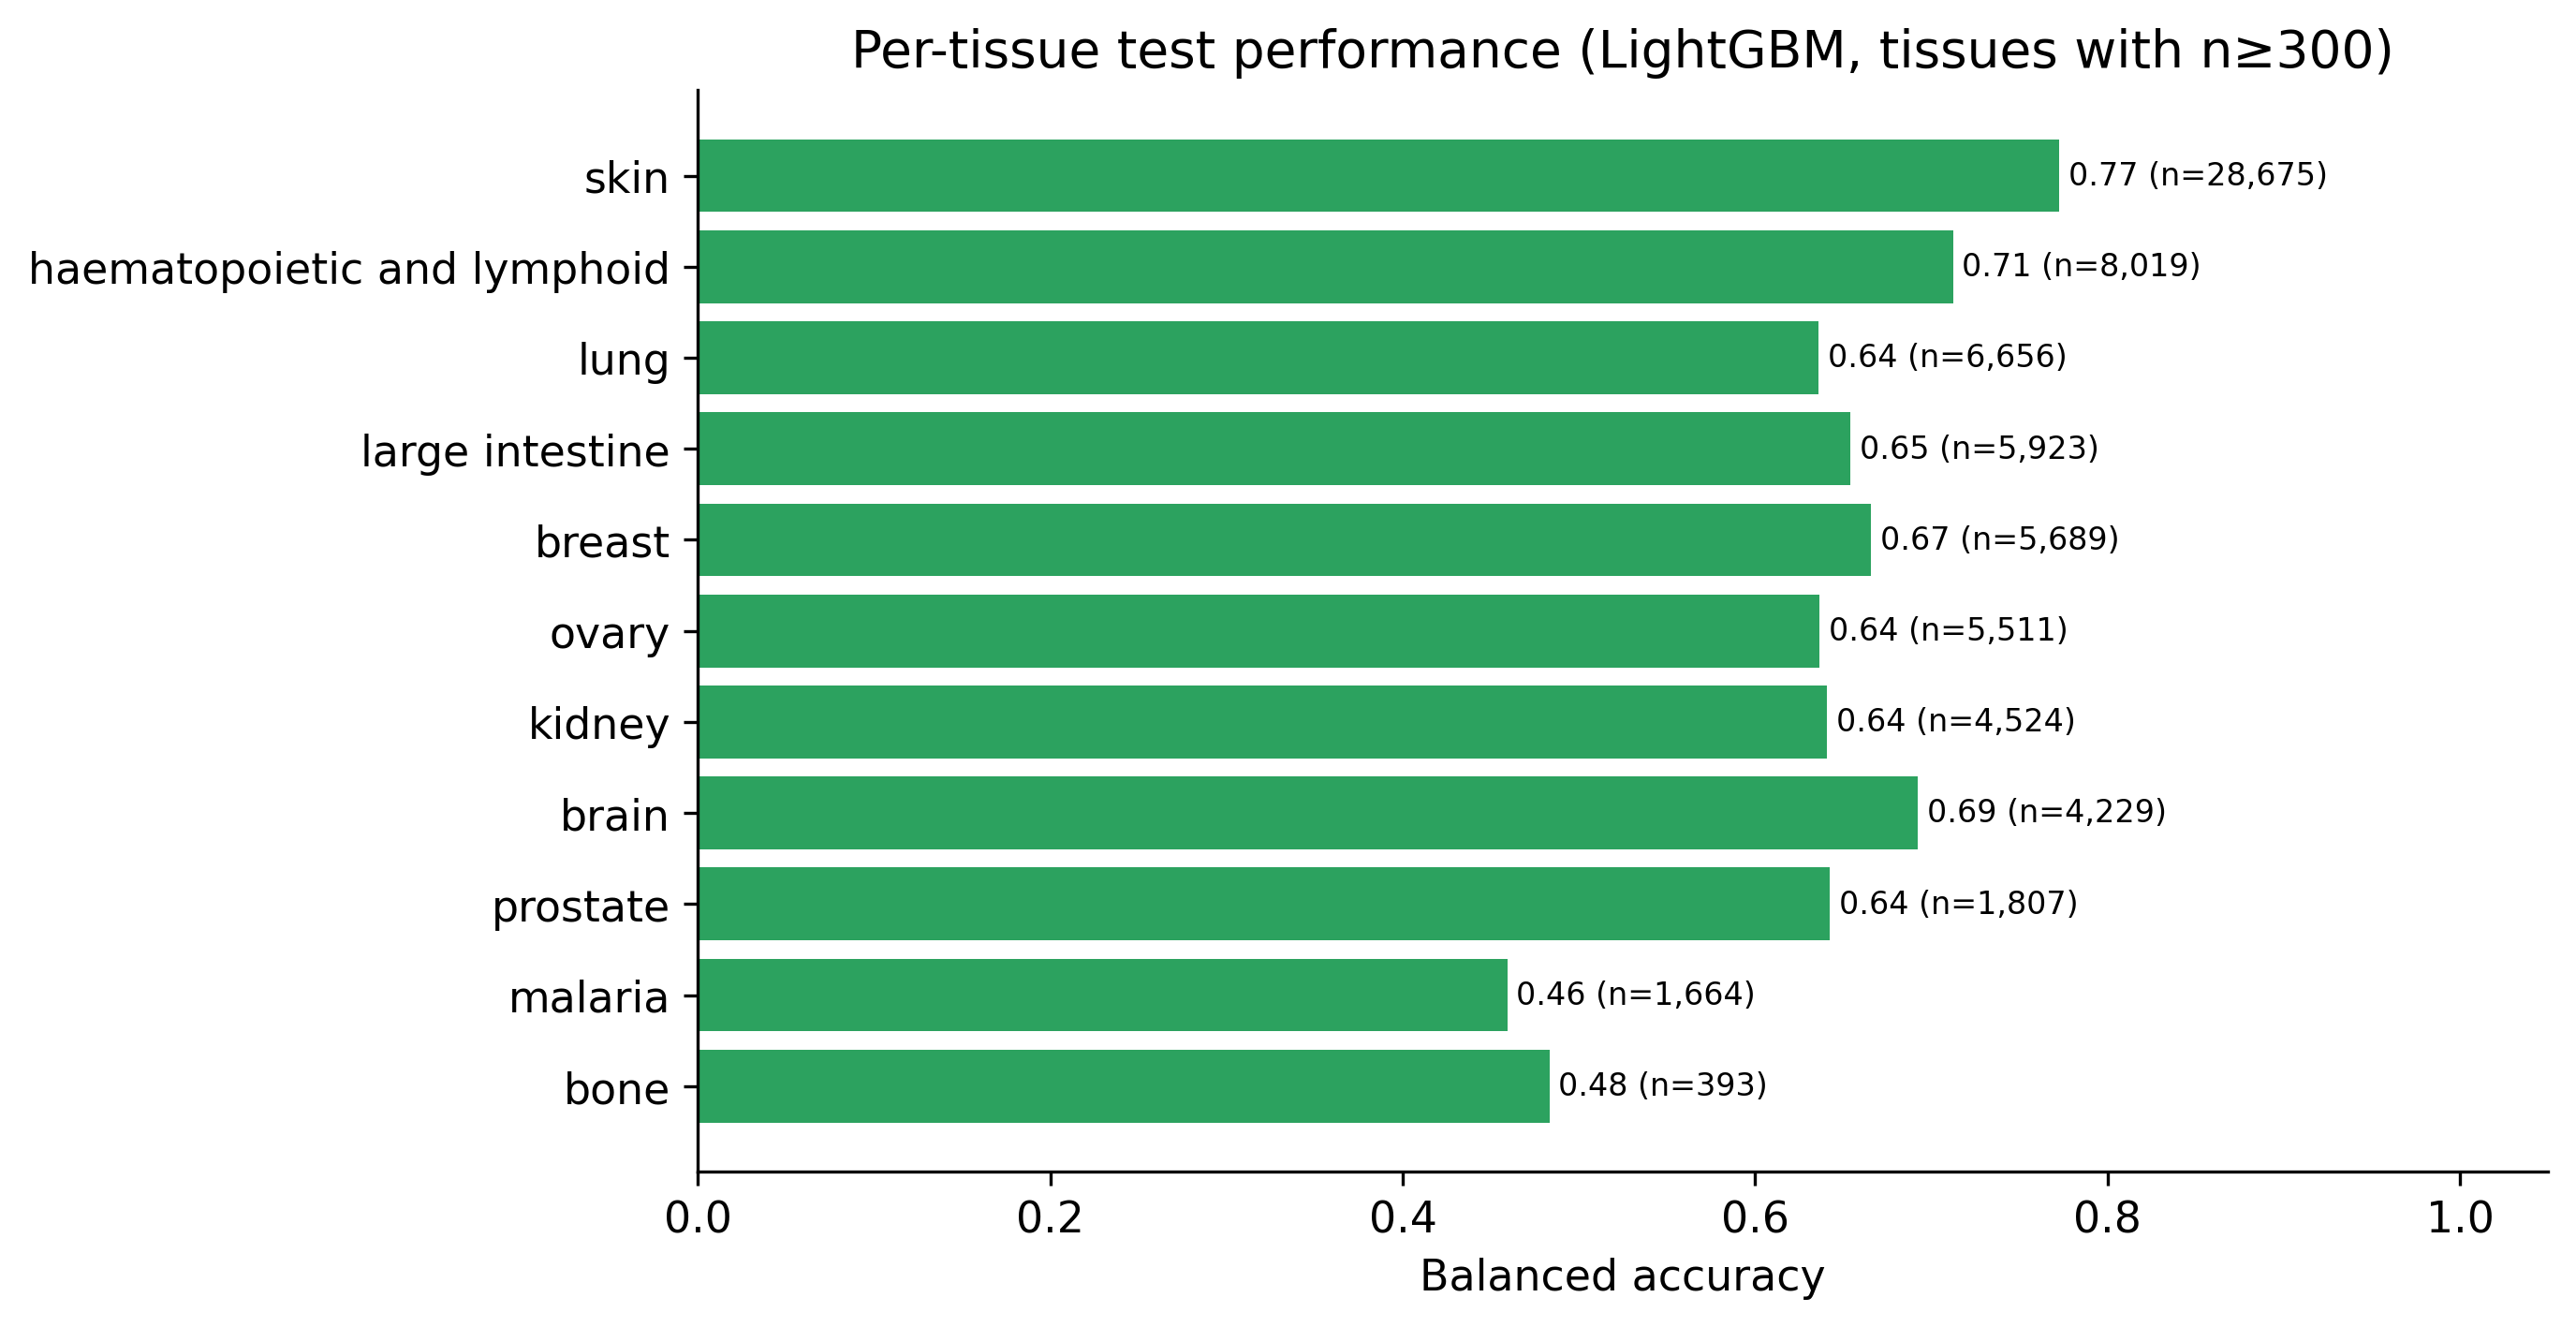
\includegraphics[width=0.8\textwidth]{fig10_per_tissue.png}
\caption{Per-tissue balanced accuracy on the standard test split (tissues with $n\geq300$ test rows).
Performance is heterogeneous across tissues.}
\label{fig:tissue}
\end{figure}

% ===================== DISCUSSION =====================
\section{Discussion}
Three findings stand out. First, drug-combination synergy class is predictable above chance from
pre-treatment descriptors alone: without chemical structures or omics profiles, a gradient-boosted
model reaches $0.805$ balanced accuracy and enriches the rare interacting classes over their priors on
a large, leakage-controlled benchmark. Second, the comparison between models is informative: the
logistic baseline clears the majority reference on balanced metrics, and the additional gains from
LightGBM ($+0.17$ balanced accuracy) do require a drug-by-cell-context interaction that no additive
model reproduces (Table~\ref{tab:baselines}). That interaction is not, however, evidence of learned
pharmacology: a smoothed per-(cell line, drug) base-rate lookup, which does nothing beyond counting
training labels, already reaches $0.778$ balanced accuracy, and the full model adds only $0.027$ beyond
it. The advantage is therefore best read as conditional memorization of entity-specific synergy rates.
Third, and most importantly, the cold-start analysis shows that this
performance does not transfer uniformly. The model is useful for novel pairings of known drugs in
known cell lines, partially robust to unseen drugs, much less reliable for unseen cell lines or unseen
tissues, and no better than chance for entirely unseen studies (Table~\ref{tab:robust}).

This reframes the result for computational-biology and bioinformatics readers. The model should not be
interpreted as a mechanistic discovery system or as a replacement for molecular-feature models. It is
a lightweight baseline and diagnostic tool: if a more complex chemical or multi-omics model cannot
improve on this benchmark, especially under leave-drug-out or leave-cell-line-out evaluation, its added
complexity is difficult to justify. Conversely, the cold-cell failure identifies the regime where
molecular and cellular features are most needed. We emphasize that the claim that molecular and omics
features would close this gap is a motivated hypothesis rather than a demonstrated result, because no
molecular model is run here; testing it directly is the natural next step.

\subsection{Limitations}
Several caveats temper interpretation. (1) Features encode identity, not mechanism; the cold-cell
collapse quantifies the resulting ceiling, and the baseline comparison in Table~\ref{tab:baselines}
shows directly that most of the standard-split performance is recoverable from conditional base rates
rather than from learned pharmacological structure. (2) Study identity may encode assay platform, dose design,
laboratory and curation effects, and should not be interpreted as a biological variable. A no-study
ablation leaves standard-split performance essentially unchanged, but leave-study-out evaluation
collapses to the random floor (Table~\ref{tab:robust}), so cross-study deployment cannot be assumed.
(3) The cold-cell collapse is largely a context effect: leave-tissue-out
evaluation, holding out whole tissues, degrades comparably (balanced accuracy $0.431$;
Table~\ref{tab:robust}), indicating limited transfer to
unseen tissues as well as unseen cell lines. (4) The dataset is composition-skewed
toward a few large screens and toward skin and blood-cancer tissues, so aggregate metrics are dominated
by those settings. (5) The ZIP score is one of several synergy definitions. The $\pm 10$ cut-off itself
is not critical---macro-F1 varies by less than $0.01$ between $\pm 5$ and $\pm 20$
(Table~\ref{tab:threshold})---but pairs near any threshold are intrinsically ambiguous, and excluding
them raises balanced accuracy appreciably, so some residual error is label noise rather than model
failure. (6) After class re-weighting the predicted probabilities remain over-confident for the rare
classes (one-vs-rest ECE $0.079$ and $0.086$ against $0.024$ overall; Table~\ref{tab:calib}), so the
scores should be recalibrated before use as absolute risks. (7) ZIP values in the source data include extreme outliers,
suggesting residual assay-quality variation that classification only partly absorbs. (8) The primary
analysis stores the two compounds in fixed slots. The audit in Table~\ref{tab:symmetry} shows this does
not inflate the reported results---removing all order-related contamination slightly improves
performance, and an order-invariant encoding costs about $0.006$ balanced accuracy---but a canonical
encoding remains preferable in deployment, and reverse-pair duplicates should be removed when the
benchmark is extended. (9) Cold-start values are summarised over a small number of entity draws
(Table~\ref{tab:multiseed}); balanced accuracy is stable across draws, but macro-AUC is more variable
and a larger number of draws would tighten these estimates.

\subsection{Future work}
The natural extensions follow directly from the limitations. The no-study, leave-study-out and
leave-tissue-out analyses reported above (Table~\ref{tab:robust}) already address the study confounder
and cross-study/tissue transfer, and the symmetry audit and multi-seed analysis
(Tables~\ref{tab:symmetry} and~\ref{tab:multiseed}) address pair ordering and holdout variability.
Remaining robustness checks are a sensitivity analysis over the $\pm 10$ classification threshold and
confidence intervals that account for clustering of rows within assay blocks and cell lines.
A natural next comparison is to reuse these exact splits with Morgan-fingerprint,
cell-line omics, molecular-image or learned graph-embedding models to quantify how much chemical
structure and cellular biology add above the identity-only ceiling, especially in the cold-cell and
leave-study-out regimes where the present model fails. Recent
multimodal, graph-based and image-based models provide natural comparators for this next
stage~\cite{monem2024,besharatifard2024,mehrabani2025}. Calibrating predicted probabilities (e.g.\
temperature scaling on a held-out fold) would make the scores usable as absolute risks, and treating
the task as ordinal regression or continuous ZIP-score prediction would better match a ranked-triage
workflow. The benchmark and pipeline released here are intended as the reference point for these
comparisons.

% ===================== CONCLUSIONS =====================
\section{Conclusions}
We presented a large-scale, leakage-controlled benchmark for classifying drug-combination synergy from
compound and cell-context descriptors on DrugComb v1.5 ($739{,}964$ combinations). A class-weighted
LightGBM model reached $0.782$ accuracy, $0.805$ balanced accuracy, $0.703$ macro-F1 and $0.922$ macro
AUC on the standard split, outperforming a logistic baseline ($p<0.001$) and enriching the rare
interacting classes over their priors. Permutation importance identified the cell line as the dominant
predictor. Crucially, cold-start evaluation revealed that balanced accuracy falls to $0.69$ for unseen
drugs, to $0.48$ for unseen cell lines, to $0.43$ for unseen tissues and to the random floor for
entirely unseen studies, exposing reliance on entity-specific information that conventional splits can
hide; a no-study ablation confirms this is not an artefact of the study identifier. The work
demonstrates that useful synergy triage is achievable for known entities without molecular features.
It also supplies a reproducible baseline against which richer models can be measured, and argues that
cold-start evaluation should be standard practice in this field.

% ===================== DECLARATIONS =====================
\section*{Abbreviations}
AUC: area under the (receiver-operating-characteristic) curve; AUPRC: area under the precision--recall
curve; CSS: combination sensitivity score; DREAM: Dialogue for Reverse Engineering Assessments and
Methods; HSA: highest single agent; IC50: half-maximal inhibitory concentration; NCI-ALMANAC: National
Cancer Institute A Large Matrix of Anti-Neoplastic Agent Combinations; OvR: one-vs-rest; RI: relative
inhibition; ROC: receiver operating characteristic; ZIP: zero interaction potency.

\section*{Ethics approval and consent to participate}
Not applicable. This study used only publicly available, de-identified in vitro drug-combination
screening data and did not involve new studies of human participants, human tissue or animals.

\section*{Consent for publication}
Not applicable.

\section*{Availability of data and materials}
The source DrugComb v1.5 summary file is publicly available from the DrugComb download portal
(\url{https://drugcomb.org/download/}) and from Zenodo record 15235991
(\url{https://zenodo.org/records/15235991}). The modeling table used in this study was generated
locally from the public DrugComb summary file using the preprocessing script described in the Methods;
no restricted or patient-identifiable data were used. The analysis code (preprocessing, training, the
three evaluation regimes, the no-study, leave-study-out and leave-tissue-out robustness experiments, a
Morgan-fingerprint structure-baseline comparator, and the bootstrap, permutation and figure-generation
scripts) and the metric outputs needed to reproduce all reported numbers are included as supplementary
material with this submission package and are intended for deposition in a public repository before
final journal submission. Programming language: Python ($\geq 3.10$). All experiments were run with a
fixed random seed ($42$).

\section*{Competing interests}
The author declares that they have no competing interests.

\section*{Funding}
This work was supported by the National Natural Science Foundation of China (grant No.~11461079). The
funder had no role in the design of the study, the analysis or interpretation of data, or the writing
of the manuscript.

\section*{Authors' contributions}
X.P. designed the study, prepared the dataset, implemented the models, performed the analysis and wrote
the manuscript. The author read and approved the final manuscript.

\section*{Acknowledgements}
The author thanks the developers and curators of the DrugComb portal for making the harmonized
drug-combination screening data publicly available.

% ===================== REFERENCES =====================
\begin{thebibliography}{99}
\small
\bibitem{holbeck2017} Holbeck SL, Camalier R, Crowell JA, et al.
The National Cancer Institute ALMANAC: a comprehensive screening resource for the detection of
anticancer drug pairs. \textit{Cancer Research}, 77(13):3564--3576, 2017.

\bibitem{oneil2016} O'Neil J, Benita Y, Feldman I, et al.
An unbiased oncology compound screen to identify novel combination strategies.
\textit{Molecular Cancer Therapeutics}, 15(6):1155--1162, 2016.

\bibitem{menden2019} Menden MP, Wang D, Mason MJ, et al.
Community assessment to advance computational prediction of cancer drug combinations in a
pharmacogenomic screen. \textit{Nature Communications}, 10:2674, 2019.

\bibitem{zagidullin2019} Zagidullin B, Aldahdooh J, Zheng S, et al.
DrugComb: an integrative cancer drug combination data portal.
\textit{Nucleic Acids Research}, 47(W1):W43--W51, 2019.

\bibitem{zheng2021} Zheng S, Aldahdooh J, Shadbahr T, et al.
DrugComb update: a more comprehensive drug sensitivity data repository and analysis portal.
\textit{Nucleic Acids Research}, 49(W1):W174--W184, 2021.

\bibitem{preuer2018} Preuer K, Lewis RPI, Hochreiter S, et al.
DeepSynergy: predicting anti-cancer drug synergy with deep learning.
\textit{Bioinformatics}, 34(9):1538--1546, 2018.

\bibitem{loewe1953} Loewe S.
The problem of synergism and antagonism of combined drugs.
\textit{Arzneimittelforschung}, 3(6):285--290, 1953.

\bibitem{bliss1939} Bliss CI.
The toxicity of poisons applied jointly.
\textit{Annals of Applied Biology}, 26(3):585--615, 1939.

\bibitem{yadav2015} Yadav B, Wennerberg K, Aittokallio T, Tang J.
Searching for drug synergy in complex dose--response landscapes using an interaction potency model.
\textit{Computational and Structural Biotechnology Journal}, 13:504--513, 2015.

\bibitem{abdelhafeez2024} Abd El-Hafeez T, Shams MY, Elshaier YAMM, Farghaly HM, et al.
Harnessing machine learning to find synergistic combinations for FDA-approved cancer drugs.
\textit{Scientific Reports}, 14:2428, 2024. doi:10.1038/s41598-024-52814-w.

\bibitem{monem2024} Monem S, Hassanien AE, Abdel-Hamid AH.
A multi-view feature representation for predicting drugs combination synergy based on ensemble and
multi-task attention models. \textit{Journal of Cheminformatics}, 16:110, 2024.
doi:10.1186/s13321-024-00903-3.

\bibitem{besharatifard2024} Besharatifard M, Vafaee F.
A review on graph neural networks for predicting synergistic drug combinations.
\textit{Artificial Intelligence Review}, 57:49, 2024. doi:10.1007/s10462-023-10669-z.

\bibitem{mehrabani2025} Mehrabani M, Lakizadeh A, Fotuhi Siahpirani A, et al.
SynergyImage: image-based model for drug combinations synergy score prediction.
\textit{BMC Bioinformatics}, 26:283, 2025. doi:10.1186/s12859-025-06314-x.

\bibitem{ianevski2020} Ianevski A, Giri AK, Aittokallio T.
SynergyFinder 2.0: visual analytics of multi-drug combination synergies.
\textit{Nucleic Acids Research}, 48(W1):W488--W493, 2020.

\bibitem{wang2026ihgcn} Wang G, Kong Y, Fu Y, Li G, Cao C.
IHGCN-PLA: an interpretable heterogeneous graph convolutional network for protein--ligand binding
affinity prediction with multimodal interaction fusion.
\textit{Journal of Biomedical Informatics}, 180:105061, 2026.

\bibitem{wang2025mmpd} Wang G, Zhang H, Shao M, Sun S, Cao C.
MMPD-DTA: integrating multi-modal deep learning with pocket--drug graphs for drug--target binding
affinity prediction.
\textit{Journal of Chemical Information and Modeling}, 2025.

\bibitem{ke2017} Ke G, Meng Q, Finley T, et al.
LightGBM: a highly efficient gradient boosting decision tree.
\textit{Advances in Neural Information Processing Systems}, 30:3146--3154, 2017.

\bibitem{pedregosa2011} Pedregosa F, Varoquaux G, Gramfort A, et al.
Scikit-learn: machine learning in Python.
\textit{Journal of Machine Learning Research}, 12:2825--2830, 2011.
\end{thebibliography}

\end{document}
